
\chapter{Reference Model Construction}
%%%%%%%%%%
\label{chap:refmod}
This chapter conceptions the process reference model and is central part of this thesis. In order to discuss particular processes, the framework itself needs to be defined. What follows is the discussion of processes \wrt to the derived process structure.

	%%%%%%%%%%

	\section{Process Framework}
	
	\citeauthor{Meise2001} defines a framework as \enquote{an ordering of relevant elements and relationships on a high level of abstraction. [...] Purpose is to give an overview about an original and to support structuring of elements and relationships on lower detail levels} \citep[\p{62}]{Meise2001}. Drawing further on his work, which especially targets framework design in process-oriented organizations, the proposed procedure for construction is adopted (\Fig \ref{fig:meise}). Differences to his approach arise, as the reference model displays an as-is state of the domain and does not follow goals of reorganization set by a specific company. Therefore, the \textit{organization} represents a fictive BPO provider in CRM, that captures derived macro structural aspects. The construction is split into two components. The structural part first encompasses strategic and fundamental reflections, while the graphical component transfers these into a visual form that supports communication.

	\begin{figure}[caption={Procedure for Framework Construction}, label={fig:meise}]
		{	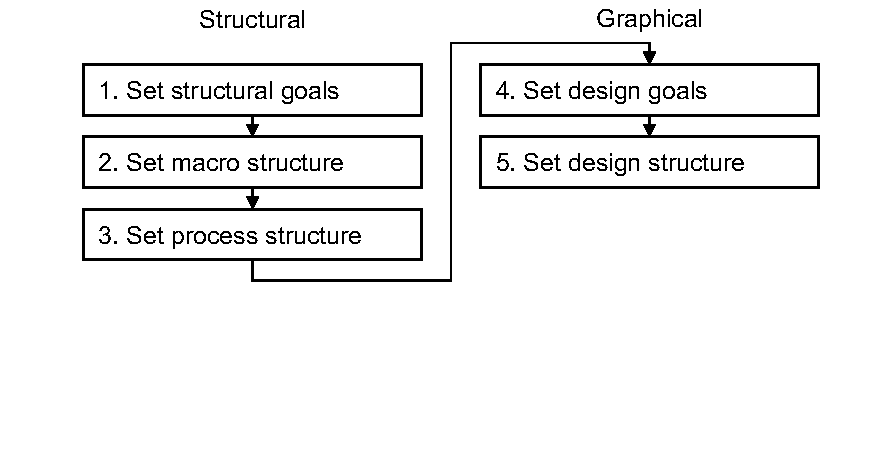
\includegraphics[width=.8\textwidth]{figures/framework-meise.pdf}}
		\parbox{0.7\textwidth }{\quelle{adapted from \citep[\p{122}]{Meise2001}}}
	\end{figure} 
	
	\subsection{Set Structural Goals}
	
	Modeling is no end in itself and different purposes require different models. Previously identified problems (\ref{sec:proide}) lead to objectives (\ref{tab:solobj}) which are to be faced with the process reference model in general and its framework in particular. The existence of general (organizational) and stakeholder-related objectives (\cf \Tab \ref{tab:solobj}) requires the framework to bring together both ends.
	
	\begin{table}[caption={Solution Objectives}, label={tab:solobj}]
		\centering
		\begin{tabular}{l p{13.3cm}}

			\textbf{No. }&\textbf{ Solution Objective}
			 \\ \hline
			\textbf{1 }                        & Construction of a generic reference model that covers distinguishing processes for BPO-providers in CRM on concept level.                                                    \\ \hline
			\textbf{2}                         & The reference model can be applied for use at Arvato CRM.                                                                                                                    \\ \hline
			\textbf{3 }                        & The construction process is well-documented, makes use of empirical research by induction, which is enriched by deduction from \acrshort{BPO} and \acrshort{CRM} theory. \\ \hline
			\textbf{4}                         & A syntactic and semantic formalized process modeling language is used, that is transferable to other languages.                                                              \\ \hline
			\textbf{5}                         & The model can be used as a statement of competence for sales activities towards clients.                                                                                     \\ \hline
			\textbf{6}                         & The model holds a process representation, which supports a common understanding across client businesses.                                                                    \\ \hline
			\textbf{7}                         & The model is able to represent an omni-channel environment.                                                                                                                 
		\end{tabular}
	\end{table}

	
	
	\subsection{Set Macro Structure}
	
	A framework incorporates concepts of strategy. One can name two perspectives, namely a market- or resource-based view of strategy, which are directed externally or internally, respectively. They are not independent of each other, but their interplay is seen as an important factor in strategic decision making and have to be considered in framework design. %Literature criticizes that standardization through reference model application has contra-productive effects on strategic competitive advantages. \cite{becker2004handelsinformationssysteme} note that the argument is true, when the reference model is used as an application model. However, the application of the reference should incorporate strategic characteristics of the company. This reference model framework is designed in a way that generic strategic orientation for providers is incorporated. 
	
	The market-based view follow the structure-conduct-performance paradigm, that explains success of a company through external factors in the industry. \cite{porter1980} formulated the so called five-forces model, which describes bargaining power of suppliers (1), threat of substitutes (2), bargaining power of buyers (3), threats of new entrants (4) and industry rivalry (5) as determinants of competition. Applying these two the BPO domain, a trivial substitute (1) for outsourced services is the return of services inside the client organization. Further, the substitution of customer services through automation may render outsourcing obsolete. The bargaining power of suppliers and buyers (3) can be loosely mapped to clients and customers. While clients as suppliers clearly influence the provider directly, customers show less of this influence on the outsourcing provider. As the provider takes an intermediate position between client and customer (\cf \Fig \ref{fig:bpochain}), their acting is always in connection with the client. However, an assessment of outsourced service quality puts pressure on the provider, which in turn will be judged by the client. The entry of new players on the market (4) can be tackled by barriers, that go back to competitive advantages of differentiation or cost-leadership. While the latter is especially causing fierce competition in low-wage regions that realize offshore-outsourcing, outsourcing players in CRM that feature more profound services lean towards a differentiation strategy. This can also be stated for Arvato. Lastly, industry rivalry (5) among players in the BPO CRM market is also influenced by the aforementioned generic strategies, to position established companies. A framework adopts market-based aspects through accounting for markets or segments therein. These are accompanied by business units or processes that relate to this external environment. 
	
	The resource-based view of strategy \citep{wernerfelt1984resource} analyzes internal strengths and weaknesses. Resources are bundled to form capabilities and should be rare, inimitable, create value and be non-substitutable. Due to asymmetries of resources, competitive advantages are enabled. The identification of capabilities of CRM BPO providers (\cf \ref{sec:bpocrmis}) can only be done on a generic level for the reference model. Application necessitates specifying the framework to conform to company-specific capabilities. The operational capability should reflect the operational process component in CRM (\cf \Fig \ref{fig:crmprocessfr}), and service delivery from the outsourcing side (\cf Appendix \ref{app:provproc}). Business development, \ie understanding and addressing client needs, misses a pendant in an isolated CRM view, but can be put in relation to delivery management in the outsourcing model. 
	
	Putting both views together emphasizes the client and customer market environment and two capabilities, that relate to these markets. %Towards the client side, providers are criticized by clients for being too reactive instead of proactive (49\%), delivering poor service quality (48\%) and lack of innovation (37\%) \citep{deloitte2014outsourcing}. While the first point of criticism addresses the client relationship, the other two are directed towards the service itself. 
	Looking at the components of \acrshort{CRM}, the people, process, technology split draws a line to the resource-based view, as these three resources need to be developed and captured to enable superior service provision for clients. Apart from the  \acrshort{CRM} view, these three also have their own meaning in \acrshort{BPO}. The importance of processes in  \acrshort{BPO} is obvious. The people component can be interpreted here as the provision of manpower and their training for services; (information) technology as an enabler of outsourcing (\cf \ref{sec:bpo}). 
	
		
	\subsection{Set Process Structure}
	\label{sec:procstr}
	Given that the model shows processes, the structural split of people, processes and technology is hardly meaningful, as two aspects of  \acrshort{CRM} or \acrshort{BPO} would be left out. Drawing from the BPO chain and the identified stakeholders (\cf \Fig \ref{fig:bpochainscope}) enables another categorization that leaves room for design choices, while capturing generic aspects of business processes within \acrshort{BPO}. As \acrshort{BPO} is the framing construct and  \acrshort{CRM} one use of it, this order is to be prioritized. The following briefly describes business processes, that are detailed in the remainder of this chapter.
	
	
	\begin{figure}[caption={BPO Chain Provider Scope with Stakeholders}, label={fig:bpochainscope}]
		{	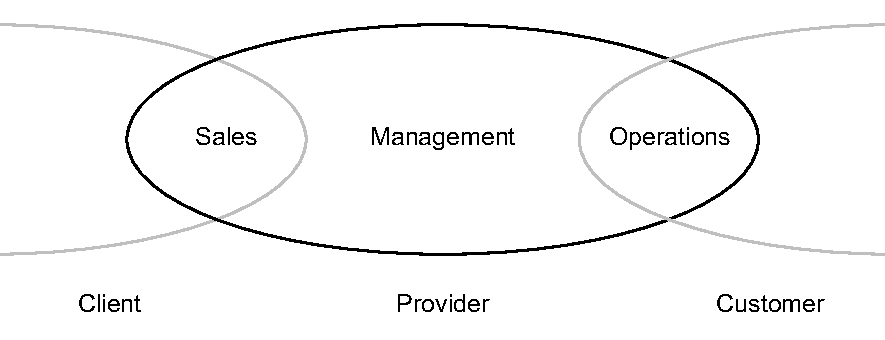
\includegraphics[width=.8\textwidth]{figures/chain2.pdf}}
	\end{figure} 
	
	\subsubsection{Sales-related}
	\label{sec:srproc}
	Sales-related processes have touch points with the client. These take place along an outsourcing lifecycle \citep{Babin_2016}.
	
	The outsourcing process is described in different frameworks in literature. \cite{perunovic2007outsourcing} investigate in outsourcing theories that cover the process as a whole and synthesize a five step process. It occurs that the greater part of frameworks take the outsourcing client's perspective, so that processes like \textit{vendor selection} or the alike are often part of frameworks. As the provider's perspective is taken in this thesis, the presented frameworks need to be examined in terms of their applicability.
	
	\cite{Agarwal_2008} present a neutral framework that is not fit on the role of the client and names activities that are driven by client and provider. From a practitioner's perspective, \cite{deloittehandbook} provide a comprehensive handbook for clients that is build around a six step process. 
	
	 %Activities prior to signing of an outsourcing contract are either driven by internal analysis in the client organization whether outsourcing is a beneficial means or an external analysis of the available providers (vendors) on the market \citep{Franceschini_2003}. 
	
	%For this agreement, the \acrshort{BPO} provider places its products in the client's requirements profile to create solutions for identified problems, noted as \textsc{Solution Design}. Also, the \textsc{Transition} and setup of the outsourced business must take place. After completion, the client relationship is maintained.
	
		\begin{figure}[caption={Outsourcing Process Framework Comparison}, label={fig:outsourcingprocesses}]
		{	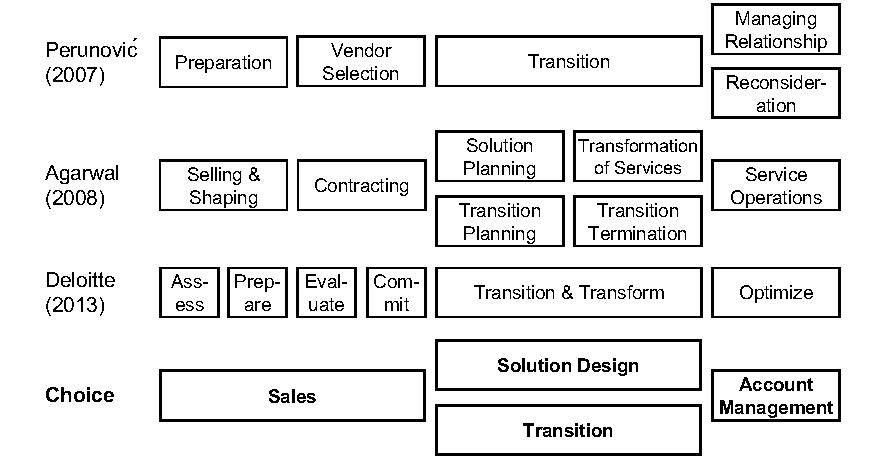
\includegraphics[width=.95\textwidth]{figures/outsourcingprocs.pdf}}
	\end{figure} 

	An intiial B2B sales process ends with a signed contract between both parties that is followed by service realization. This is chosen to be modeled in a single \textsc{Sales} process (\cf \Fig \ref{fig:outsourcingprocesses}), as the split into multiple components is motivated by (client)-internal steps prior to the approach of potential vendors. 
	
	The realization of the outsourcing agreement can be split into two streams \citep{Agarwal_2008}. On the one hand there is the creation of the provider's solution that addresses the client's problem. The solution relates to the provider's product portfolio and its application. On the other hand, the client needs to pass over the existing in-house business to the provider in order to realize the outsourcing. These two aspects are separated into the two processes \textsc{Solution Design} and \textsc{Transition}. The former ends with the service's implementation for the client, while the latter is completed with all new services being live and operational. The interdependency of these two is visualized by their parallel arrangement. 
	
	The last part of the examined outsourcing frameworks characterizes activities that take place after \textsc{Transition}. From a provider perspective, this follow-up can be described as client relationship maintenance \citep{Moncrief_2005}. 
	To avoid confusion through naming and emphasizing the relationship's B2B-aspect, \textsc{Account Management} is chosen as the label for the fourth main process.

	
	
	\subsubsection{Management-related}
	The management-related business processes bring together resources in the provider organization, so that the operations and business development capability are realized. Regarding the latter, it is important to have a products in place, which can be implemented as service solutions for clients. \cite{schewe2007} names this delivery management, but explicitly refers to its similarities with product development. In addition to the development, the management of existing products inside a product portfolio becomes important. These two processes shall be called \textsc{Product Development} and \textsc{Portfolio Management}.
	
	Benefits through economies of scope are a question of offered services. The operations capability can be addressed by processes that enable economies of scale. These are realized by the increased output of services across client businesses, which in turn necessitates alignment in these services so that their output can be counted \textit{together} (\eg thereby enabling economies of scale). This alignment is facilitated through a product-view of services and their underlying portfolio in the organization. Moreover, service quality must be assessed to assure conformity with client agreements, as well as in terms of internal improvement and benchmarking. This is represented in the \textsc{Quality Management} process. 
	
	In addition, people in the provider organization need to be trained in order to excel in their role as \acrshort{CSR}. Their career path can be seen from a process perspective, so that a strong relationship is established with their employer. This aspect shall be called \textsc{People Lifecycle Management}\footnote{The term people is preferred over agent or \acrshort{CSR}, because it puts this process strongly in connection \acrshort{CRM}. As the management-related processes are tried to be referential for \acrshort{BPO} in general, this is not intended.}. 
	
	Lastly, management of service delivery, especially scheduling, becomes critical in a business like customer service. The assurance of the right capacity at the right time to meet fluctuating demand with little waiting time is expected from the client. Therefore, efficient techniques to manage the complexity of multiple channels, different demand patterns and different skilled \acrshort{CSR}s are necessary. This is encapsulated in  \textsc{Operations Management}. 
	
	\subsubsection{Operations-related}
	The last group of business processes target the service delivery in the words of \citeauthor{schewe2007}. The processing of transactions with customers is in focus, which can be on numerous channels. In this case a transaction is a conversation, so that theories of communication \citep{shannon1949} shall be applied. A message is sent from a sender to a receiver through a medium. In case of customer service, both the customer or the \acrshort{CSR} can start a conversation, that has a subject which relates to the client in some way. Reasons for contact may be separated by being related to a previous transaction. This transaction might be a purchase of a client's good or service. The communication channel increasingly varies and is intended to be no obstacle in an omni-channel environment, because it is strived for a seamless experience across channels. Hence, processes should be similar before going into technical details. 
	
	Communication can be asynchronous (\eg, e-mail) or synchronous (\eg, voice), which puts emphasis on temporal differences in the conversation. While the employed process definition encompasses the \enquote{time-logical sequence of activities}, the value (\viz time between activities) does not impact the process logic itself, as this is a question of succession. General steps in inquiry handling from a business perspective will be similar independent of the (a)synchronous case. What becomes more important from a business perspective is the question concerning the contact initiator. A communication triggered by the customer (incoming) follows demand patterns that are inferred from historic data, while better planning of \acrshort{CSR} opened contacts (outgoing) is possible, as the temporal decision of contact lies at the business and not the customer. These two ways are represented by the \textsc{Inbound} and \textsc{Outbound Services}.
	
	Lastly, one has to differentiate in customer contact whether \acrshort{CSR}s are involved in inquiry handling, which obviously has business implications. When customers use self-service to address their needs, software takes the \acrshort{CSR} role, which saves resources. Providers can differentiate themselves through expertise in these systems. Clients save money by less volume that is processed by humans (employees of the outsourcing provider). At first sight, this may cannibalize outsourcing business, but the expertise of installing and running these self-service systems is likely not located in clients that outsource \acrshort{CRM}. Consequently, providers can generate new business by accumulating know-how in \textsc{Self-Services}. 
	
	On the one hand, they design the customer-facing self-services in order to handle inquiries. On the other hand, the provider manages and maintains the knowledge base, that is located behind these automatons in the back-end. This does not only have implications on self-services, but also on other customer contacts, as the \acrshort{CSR}s in the human-to-human communication also query the knowledge base to solve customer problems. The \textsc{Knoweldge Management} process models these aspects.
	
	It is desisted from the explicit modeling of a customer journey, because it encompasses components that cannot be part of a process model for providers. The model in this thesis is centered on the outsourcing provider. Modeling of a customer journey requires a customer-centric model, which then contains steps of the customer journey in a detailed way. Such a model should be a \textit{playground} for identifying space for improvement in dialog with a client regarding its customer journey. In addition, it would benefit from avoiding the standards of process models, as its purpose is seen in the \textit{design} of a journey through \acrshort{CRM} components. Research from the field of marketing can be a starting point \citep{Lemon_2016, Frow_2007}. 
	
	\subsection{Set Design Goals}
	
	The visual representation of the framework is linked to its cognition among viewers, therefore it needs to support the communication of the reference model's purpose. In contrast to language-processing, the process of perception is foregrounded, as the graphic is processed all at once and not sequentially. The model has to capture the fundamental characteristics of the domain of outsourcing at first glance. The sketched model level when applied (provider and client model) should be visually supported, as the reference model's framework is the blueprint to convey this hierarchy. 
	
	\hfill\begin{minipage}{\dimexpr\textwidth-1.2cm}
		\textbf{Design Goal 1}: The framework has to visualize the business of BPO providers.
	\end{minipage}

From a process perspective, as well as to reduce complexity, it helps to highlight important core processes over supporting or coordinating processes. By doing this, the viewer gets an impression about central parts of the model. 

	\hfill\begin{minipage}{\dimexpr\textwidth-1.2cm}
	\textbf{Design Goal 2}: The framework has to distinguish core processes from other process types. 
\end{minipage}

Furthermore, provisioned service types are to be shown. In order to gain an understanding of characteristics in CRM outsourcing, especially in an omni-channel context, the framework has to clearly communicate customer orientation. As it is the differentiating aspect towards BPO for other processes, this fact should be incorporated in design.  

	\hfill\begin{minipage}{\dimexpr\textwidth-1.2cm}
	\textbf{Design Goal 3}: The framework has to cover the CRM-orientation in service provision. 
\end{minipage}

A framework's purpose is to manage complexity by displaying relevant elements. In addition, the visual representation should be clear, consistent and structured to enable understanding on its own. 

	\hfill\begin{minipage}{\dimexpr\textwidth-1.2cm}
	\textbf{Design Goal 4}: The framework has to be easily processable by viewers without further explanation. 
\end{minipage}

	\subsection{Set Design Structure}
	
	The design of the reference model primarily addresses reference model users. However, its design will have large influence on the depiction of an application model. It is noted that the framework is designed independent of a process modeling language. The use of a reference design (model) can serve as a basis, as it includes benefits that have been previously discussed in context of reference models. The house reference design for example is used in the Retail-H (\cf \ref{mod:retail}).
	
	Known patterns influence human perception \citep{kroeber1997} and can transfer associations. In case of the house reference design, one can link solidity, stability and security \citep[\p{216}]{Meise2001} with it. It consists of three parts (roof, core, foundation), which can be used to visualize coordination, main and supporting processes, respectively. The foundation represents a basis on which the house is built. Its main part, biggest in size, stands in center and has the largest impact on the perception of the house's content. The roof brings together underlying elements and has an analogy towards an organizational hierarchy. 
	
	\subsubsection{Framework composition}
	
	Adding the previously discussed process structure, supported by the BPO-chain design, one can convey this representation into the core area. \Fig \ref{fig:frameworkdesign} shows influences for the framework components. 
	\citeauthor{Meise2001} proposes the use of a value chain representation with a chevron that enables linking of multiple elements, which is called a \acrfull{VACD}. It communicates the input, transformation, output relation of a company, as the area on the left or right hand side of the house can be used to model supply or distribution markets. 
	These two markets are existing in BPO with end-customer interaction, which brings together house reference design and \acrshort{BPO}-chain. 
	
	\begin{figure}[caption={Framework Design Influences}, label={fig:frameworkdesign}]
		{	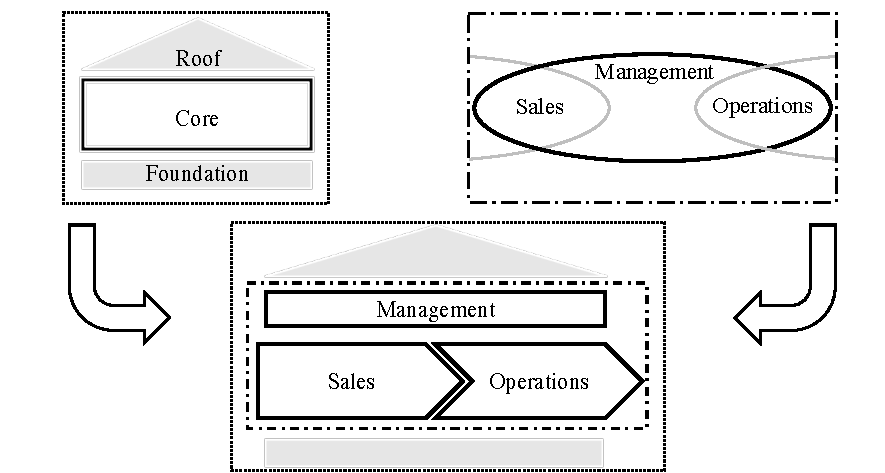
\includegraphics[width=.8\textwidth]{figures/frameworkdesign.pdf}}
	\end{figure} 
	
	
	The value chain can be represented by the exclusive use of chevrons that are linked together or it can have one starting element, which is a pentagon. This element is \textit{closed} to the left side. Porter uses the \textit{closed} variant, where the widened interface to the left side is emphasized. As the left side of the framework represents the client side, the strong link to the outsourcing partner shall be highlighted \wrt the customer-facing right hand side. Here, the interface to the customer shall be pointed for the following reasons. First, the interaction with a customer is intended to be independent of communication channel, so that the idea of omni-channel is conveyed (and with it the \textit{one face to the customer}- and \textit{one face of the company}- paradigm). Second, the customer's importance is communicated with this representation, as all action (complete height of the chain) is pinpointed towards one customer. The  process structure consequently locates sales processes on the left and starting part of the value chain and connects the operations processes with it to address the two markets. 
	
	The management processes are located in the bar above the value chain. While it is part of the house's core, it does not have a \acrshort{VACD} representation, as it has little contact with clients or customers. However, it influences the complete part of business and is a indispensable part of the \acrshort{BPO} provider business, hence it must be part of the core instead of the roof. Sales-related processes benefit from \textsc{Product} and \textsc{Portfolio Management}, while \textsc{People Lifecylce Management} and \textsc{Operations Management} are scoped towards service delivery and with it operations. \textsc{Quality Management} is expected by clients, but also important for the provider organization as a whole. Hence, it is located in the center of the upper management processes. Reason for locating the bar at the top of the \acrshort{VACD} is that these processes include tactical to strategical aspects, that influence the underlying processes in the framework's core. 
	
	\subsubsection{Framework details}
	
	Locating the identified processes on the framework needs to be done carefully, as their position and shape is important for the viewer's perception. The three areas of the framework's core narrow down positioning alternatives. Their size and shape is equal, to emphasize their main process feature. Customer facing processes vary slightly. Support and Coordination processes have a smaller boxes, font size and slimmer boarders to limit their attention. \Fig \ref{fig:framework} shows the framework.
	
		\begin{figure}[caption={Framework}, label={fig:framework}]
		{	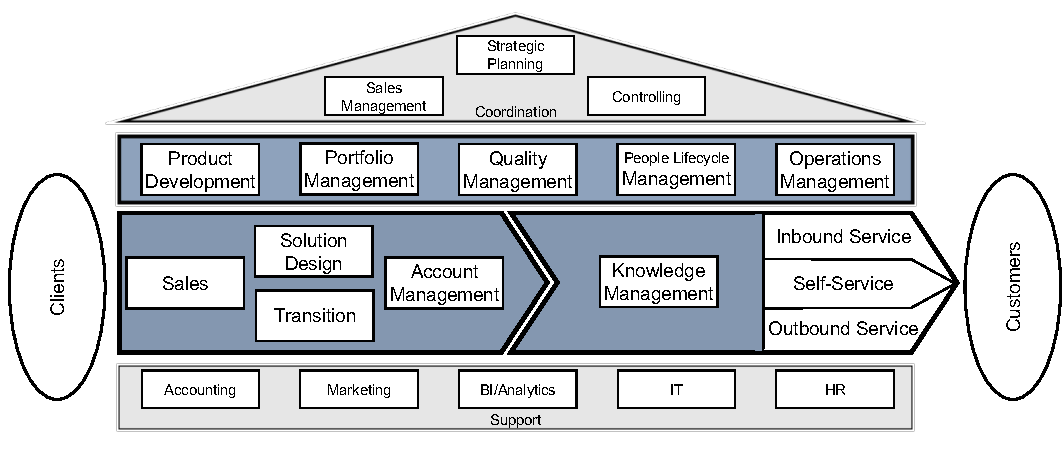
\includegraphics[width=.99\textwidth]{figures/framework_full.pdf}}
	\end{figure} 
	
	
	 Starting with sales-related processes, the main processes \textsc{Sales}, \textsc{Solution Design}, \textsc{Transition} and \textsc{Account Management} have to be placed on the framework. As explained in \ref{sec:procstr}, they follow a lifecycle, so that \textit{Sales} leads to \textit{Solution Design} and \textit{Transition}, while existing clients relationships are cared in Account \textsc{Management}. This leads to a positioning of \textsc{Sales} as the leftmost and \textsc{Account Management} as the rightmost process within the sales area. \textsc{Transition} and \textsc{Solution Design} are processes that take between the previous ones. They are both part of a client business setup and are hence located next to each other. todo{bpo lifecycles, wiederholung zu später}
	 
	 Operation-related processes have the peaked customer interface as starting point for locating processes. These are split into \textsc{Inbound Service}, \textsc{Outbound Service} and \textsc{Self-Service} as customer-facing processes, that are accompanied by \textsc{Knowledge Management} as a process that takes place in background. Consequently, \textsc{Knowledge Management} is located towards the center of the framework and not directed to the customer. The other three processes share their direct customer contact and are therefore in the right part of the chevron. To emphasize their role as the interface to the customer, their representation is adjusted to link to the customer. Furthermore, they are also located on the same height in the chains flow to highlight that these are alternatives of contact. By making no distinction of channels on framework level, their equality of treatment is represented. 
	 
	 Five management processes are located next to each other in their area on top of the \acrshort{VACD}. The product and portfolio processes have higher connection to the client side, as these service products are sold to clients. The \textsc{Product Development} process has a stronger external relation, as new products should meet unsatisfied demands from the market. \textsc{Portfolio Management} on the other hand is an intra-organizational process that sets its focus on the provider. \textsc{Quality Management} is centered and subject to client businesses as well as internal management. The other two processes, namely \textsc{People Lifecycle Management} and \textsc{Operations Management} impact \acrshort{CSR}s and service delivery. Their positioning can be reasoned through an higher impact of \textsc{Operations Management} on the service delivering activities through schedules, plans and forecasts of customer demand. \textsc{People Lifecycle Management} on the other hand is again oriented towards the provider organization, because management of human resources for service delivery is of direct interest for the provider, but not to the customer.
	 
	 Support and coordination processes are not further specified in this thesis. Their elements are inspired by general processes that also play a role in \acrshort{BPO} and other the retail-H reference model \cite{becker2004handelsinformationssysteme}. The \textit{Accounting} process fulfills the task of keeping financial accounts. \textit{Marketing} as a support process is narrowly defined as the positioning of the provider towards the client market for example by means of advertisements. Strategic and managerial aspects are captured in Sales Management. 
	 
	 \textit{ \acrfull{BI} / Analytics} captures the process of supporting the business through data-driven insights, as well as to provide decision-support for management on a tactical or strategic level. The latter emphasizes especially the \acrshort{BI} aspect and would also make a positioning in the roof considerable. However, apart from the management reporting function, \acrshort{BI} can also be seen on an operational level. Recently, the notion of analytics become popular. No clear border between the two fields can be defined in the literature \citep{mertens}. \cite{Chen:2012:BIA} suggest the term \textit{\acrshort{BI} \& Analytics}, which is used here. Interpretation of the two notions will vary in an application, as it depends on the understanding in the target provider organization. 
	  
	  \textit{IT} supports business through operation of systems (for instance in accounting, HR or for decision-support in management). \textit{HR} manages people in the provider organization and is different from People Lifecycle Management, as it focuses on  employees in operational service delivery, not personnel management in general. 
	  
	  \textit{Sales Management} as a coordination process is subject to planning of client businesses and verticals. It is located on the left side of the roof to move it closer to the sales processes. \textit{Strategic Planning} guides the provider organization as a whole with a long-term perspective. It is located highest in the roof to emphasize its importance for the strategic management of the organization. \textit{Controlling} completes the coordinating processes by supplying the management with information and overseeing the client businesses. 
	 	 
	 \subsubsection{Addressing  Design Goals}
	 
	 	 	\begin{table}[caption={Design Goals}, label={tab:desobj}]
	 	\centering
	 	\begin{tabular}{l p{13.3cm}}
	 		
	 		\textbf{No. }&\textbf{ Design Goal}
	 		\\ \hline
	 		\textbf{1 }                        & The framework has to visualize the business of BPO providers.                                     \\ \hline
	 		\textbf{2}                         & The framework has distinguish core processes from other process types.                                                                                                                   \\ \hline
	 		\textbf{3 }                        & The framework has to cover the CRM-orientation in service provision. \\ \hline
	 		\textbf{4}                         & The framework has to be easily processable by viewers without further explanation.                                                              
	 		
	 	\end{tabular}
	 \end{table}
 
	 
	 With the proposed framework shown in \Fig \ref{fig:framework}, the four design goals are achieved. Its fundamental structure with the \acrshort{VACD} shows encapsulates the BPO business and by exchange of the right chevron, one can apply the model to other BPO domains than \acrshort{CRM}. The relevance of core processes is highlighted through use of the house reference design and coloring. The right chevron is suited to represent service delivery in \acrshort{CRM} through focus on customer contact, while abstracting from explicit processes for offered services (products). These are contained in the \textsc{Product Development}, \textsc{Solution Design} and \textsc{Portfolio Management} process without specifying of measures. Naming these would conflict with the intent of a reference model, as these will be different for companies in the domain. A minimalistic two dimensional representation without additional distracting features such as  varying fonts supports effortless understanding of the framework. The different shapes are limited and the use of rectangles is preferred. Other elements, like the \acrshort{VACD}, are associated by the viewer and naturally convey the flow of the framework: the outsourcing client's \acrshort{CRM} is given to the provider, who then adds the value to the chain and sends it to the customer. It is noted that application of the reference model results in differences in content, but also in design (to conform to corporate design for instance). However, a post-design evaluation of this framework design was not conducted, so these conclusions reflect the author's intentions.
	 
	 The following dives into the process models below the framework. The icebricks language is used to meet solution objective 4 and hence the underlying structure below the main processes on the framework is composed of detail processes, which in turn have process building block underneath. 
	 
	 
	 %%%%%%%%%%
	 \section{Customer Processes}

	 
	 This section describes the \textsc{Inbound Service}, \textsc{Outbound Service}, \textsc{Self-Service} and \textsc{Knowledge Management} process. They represent the operational transaction processing in outsourcing and are driven by the target domain (\acrshort{CRM}). 
	 
	 There are several entities that encompass all means of contact to the outsourcing provider. First, every contact involves a customer asking for something or having a lack of information that is to be addressed. This lack is possibly related to a product\footnote{Product here encompasses everything that is provided by the client to the market, \ie, services as well.} of the client (be it an actual purchase or solely the consideration), which is denoted as a transaction. Transactions also cover touch points like past customer service contacts or other events between the customer and the company. Together, these product-related and touch point-related transactions are determinants for forming a complete view of the customer. Transactions have a hierarchy, so that one transaction may have to a superior transaction. 
	 
	 Here, it is assumed that every transaction is related to a customer. Even considering a new customer, the act of contacting implies a previous touch point with the company. It is noted that this transaction might be not known to the company. A customer can have multiple transactions. The contact happens as an \textsc{Inbound Service } (customer contacts company), \textsc{Outbound Service} (company contacts customer) or\textsc{ Self-Service} (customer reaches company without involvement of a \acrshort{CSR}). 
	 
	 Knowledge bases accessible by the outsourcing provider contain knowledge which support addressing the customer's issue that is reason for contact. As these issues are classifiable, structuring them leads to business cases that describe the solution to a known customer problem. Examples can the cancellation of a booking, the termination of a contract or change of address. This listing reveals that business cases are very dependent on the business of the client and hence are not a valid criterion for structuring customer contacts in a reference model. Not every customer contact needs to relate to a case. The \acrshort{ERM} in \Fig \ref{fig:contacterm} shows the described circumstances around the contact. It also reasons the structuring of the later described \textsc{Knowledge Management} process. 
	 
	 \begin{figure}[caption={\acrshort{ERM} of Customer-facing Services}, label={fig:contacterm}]
	 	{	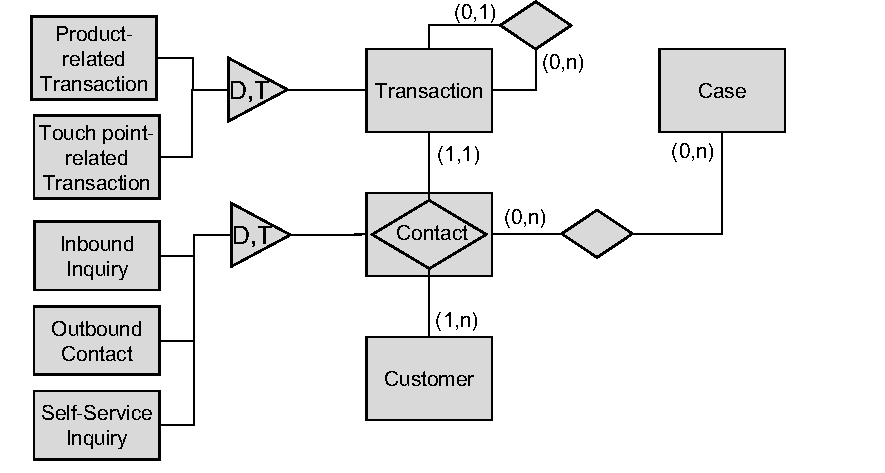
\includegraphics[width=.8\textwidth]{figures/contacterm.pdf}}
	 \end{figure} 
	 
	 
	 %hippner:692 muss nicht nur inbound sein, outbound geht auch
	 
	 \subsection{Inbound Service}
	 \label{pr:inb}
	 The associated object to this process in the \textit{inquiry}\footnote{inquiry is American English; enquiry is British English.}. It is preferred over \textit{request} as it emphasizes an investigation in an issue over the politeness during asking. It is defined as an act of asking for information \citep{oxfordenquiry, oxfordrequest}. In this case, it is the customer who is lacking information in some regard and contacts the company. A \acrshort{CSR} of the outsourcing provider attends to the matter. 
	 
	 Reflections on the structure of the process become especially important in case of an omni-channel environment. There are multiple contact channels, asynchronous and synchronous communication and generic reasons that lead to the inquiry. Rationale behind omni-channel process modeling must be to keep the structure channel independent as long as possible to enable alignment. To capture the peculiarities of the channels, the concept of (detail process) variants is used on the lowest level to distinguish between mail, voice, direct messenger and social channels. Reasons for this split is that other discussed channels (video, website, app) can be included in others by means of a process view (video to voice) or are not a contact channel by means of inbound customer service. A website or app is a gateway to other channels (\eg, direct messenger) or to self-service, but do not offer direct engagement with a \acrshort{CSR}. Variants can also be added, so that new channels can be integrated to the model without causing structural conflicts. While there are similarities between (a)synchronous channels, using these as variants forecloses capturing of channel idiosyncrasies, because the underlying process building blocks would be the same for a variant. 
	 
	 Based on insights of the process modeling workshop, the detail processes are structured so that their steps apply to all channels and is shown in \Fig \ref{fig:inbproc}. First, the detail processes are described without going into details of their channel-variants, then each detail process is described \wrt the four variants. 
	 
	 \begin{figure}[caption={\textsc{Inbound Service} Process}, label={fig:inbproc}]
	 	\begin{subfigure}[b]{.45\textwidth}
	 		\begin{center}
	 			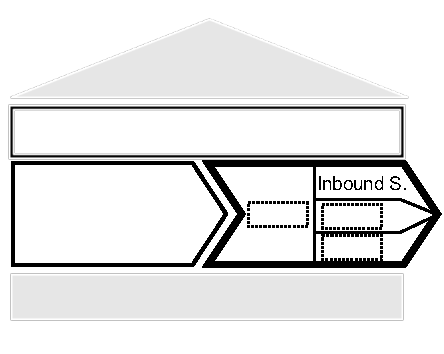
\includegraphics{figures/processes/inbound.pdf}
	 		\end{center}
	 	\end{subfigure}
	 	\begin{subfigure}[b]{.45\textwidth}
	 		\begin{center}
	 			\begin{tikzpicture}
	 			[node distance=.4cm, start chain=going below,font=\sffamily]
	 			\node[punktchain, rounded corners=0pt, join=by {-}] (eins)      {route inquiry};
	 			\node[punktchain, rounded corners=0pt, join=by {-}] (zwei) {preprocess inquiry};
	 			\node[punktchain, rounded corners=0pt, join=by {-}, ] (drei) {classify inquiry};
	 			\node[punktchain, rounded corners=0pt, join=by {-}, ] (vier) {process inquiry};
	 			\node[punktchain,rounded corners=0pt,  join=by {-}, ] (fuenf) {review inquiry};
	 			\end{tikzpicture}
	 		\end{center}
	 	\end{subfigure}
	 	
	 \end{figure}
	 
	 First, an inbound inquiry is initiated by a customer and the connection with the receiving end is established. Before an interaction starts, the inquiry needs to be guided to a \acrshort{CSR}, which is known as routing in telecommunications. During this \textit{routing} process, information from the customer is processed, so that part of his needs can be inferred before the employee starts the communication and time (and money) is consumed. Time that the customer spends in the system before the communication starts is not consuming resources from the provider, so the pre-extraction of information usable to address his problem is desirable. At the end of routing, a \acrshort{CSR} is found that starts the communication with the customer. In the \textit{preprocessing} step, the \acrshort{CSR} takes on the inquiry and consumes the information that is available from routing, as well as transmitted by the customer. After this familiarization the \acrshort{CSR} can \textit{classify} the \textit{inquiry}, so that it is known how to map the individual inquiry of the customer to a case (if existent). The \textit{process inquiry} detail process engages the inquiry and ideally solves the problem. The last step involves a \textit{review} and closes the interaction. It updates data related to the communication and stores it in the knowledge base. As every detail process in \Fig \ref{fig:inbproc} has four variants, these are shown one by one in the following. 
	 
	 \subsubsection{Route Inquiry}
	 
	 Going into the specifics of the route inquiry detail process, \Fig \ref{fig:inbound:route} shows its four variants consisting of process building blocks. One can observe similarities 
	 across all variants especially at the beginning and end. During routing, no \acrshort{CSR} is actively involved.
	 \\
	 
	 \begin{figure}[caption={Route Inquiry Detail Process}, label={fig:inbound:route}]
	 	
	 	\begin{subfigure}[b]{.45\textwidth}
	 		\centering
	 		\begin{tikzpicture}
	 		[node distance=.4cm,
	 		start chain=going below,font=\sffamily]
	 		
	 		\node[punktchain, join=by {-}] (eins)      {determine language};
	 		\node[punktchain, join=by {-}] (zwei) {analyze inquiry};
	 		\node[punktchain, join=by {-}, ] (drei) {priorize inquiry};
	 		\node[punktchain, join=by {-}, ] (vier) {select CSR};
	 		\node[punktchain, join=by {-}, ] (fuenf) {route inquiry};
	 		\node[punktchain, draw=white] (sechs) { };
	 		
	 		\end{tikzpicture}
	 		
	 		\caption{Mail Variant}\label{fig:inbound:route:mail}
	 	\end{subfigure}
	 	\begin{subfigure}[b]{.45\textwidth}
	 		\centering	
	 		\begin{tikzpicture}
	 		[node distance=.4cm,
	 		start chain=going below,font=\sffamily]
	 		
	 		\node[punktchain, join=by {-}] (eins)      {determine language};
	 		\node[punktchain, join=by {-}] (zwei) {analyze inquiry};
	 		\node[punktchain, join=by {-}, ] (drei) {analyze environment};
	 		\node[punktchain, join=by {-}, ] (vier) {priorize inquiry};
	 		\node[punktchain, join=by {-}, ] (fuenf) {select CSR};
	 		\node[punktchain, join=by {-}, ] (sechs) {route inquiry};
	 		
	 		\end{tikzpicture}
	 		\caption{Social Variant}\label{fig:inbound:route:social}
	 	\end{subfigure}
	 	\begin{subfigure}[b]{.45\textwidth}
	 		\centering	
	 		\begin{tikzpicture}
	 		[node distance=.4cm,
	 		start chain=going below,font=\sffamily]
	 		\node[punktchain, draw=white] (null) { };
	 		\node[punktchain] (eins)      {determine language};
	 		\node[punktchain, join=by {-}] (zwei) {collect IVR data};
	 		\node[punktchain, join=by {-}, ] (drei) {select CSR};
	 		\node[punktchain, join=by {-}, ] (vier) {route inquiry};
	 		
	 		\end{tikzpicture}
	 		\caption{Voice Variant}\label{fig:inbound:route:voice}
	 	\end{subfigure}
	 	\begin{subfigure}[b]{.45\textwidth}
	 		\centering	
	 		\begin{tikzpicture}
	 		[node distance=.4cm,
	 		start chain=going below,font=\sffamily]
	 		\node[punktchain, draw=white] (null) { };
	 		\node[punktchain] (eins)      {determine language};
	 		\node[punktchain, join=by {-}] (zwei) {analzye inquiry};
	 		\node[punktchain, join=by {-}, ] (drei) {select CSR};
	 		\node[punktchain, join=by {-}, ] (vier) {route inquiry};
	 		
	 		\end{tikzpicture}
	 		\caption{Direct Messenger Variant}\label{fig:inbound:route:dm}
	 	\end{subfigure}
	 \end{figure}
	 
	 A common language is a requirement for any communication and needs to be known to understand the content of the inquiry. While this is required across channels, differences arise in the following step: All variants except voice can analyze the inquiry. This analysis uses available information from the inquiry, \ie its content or channel-specific data to identify the customer and infer the customer's need. In voice the inquiry itself is not existent at this point, as the customer has not expressed it verbally. However, \acrfull{IVR} technology helps to extract information from the customer without active involvement of a \acrshort{CSR} and is a typical technology in contact centers \citep{Thomas:2009}. The distinction between voice and the other variants is reasoned by the fact that the other inquiries are text-based and therefore analyzable by common means. As \acrshort{IVR} is a standard in customer service, the naming of a explicit technology does not create conflicts in terms of universal applicability. The amount of information processed varies: Simple systems might just record input from the customer typed in via the phone keypad (\textit{if you have  a question regarding X, please press 2}), while sophisticated systems do natural language processing.
	 
	 The social variant includes an \textit{analyze environment} building block, which emphasizes the importance of the network's context in social media. The verb \textit{analyze} is again used to state automatism in this step. 
	 
	 Asynchronous channels (\ie, mail, social) have a \textit{priorize inquiry} step, that work around simple \acrfull{FCFS} processing of inquiries. This step is not seen for synchronous channels, as the customer actively waits for a \acrshort{CSR} to take care of the inquiry. However, \textit{select \acrshort{CSR}} can take several aspects into account that influences whether a suitable \acrshort{CSR} is available:
	 Requirements of the inquiry (\ie, language and to that point known content of the inquiry) and status of the customer (if known) are two examples . 
	 
	 Means to narrow down the variety content-wise is the availability of different contact channel instances. For example, there could be a dedicated mail address for reservations and another one for bookings. The fit of inquiry requirements to agent skills is known as skill-based routing. \acrshort{CSR}s can be clustered in agent groups that are the right contact person for the inquiry, so that additional rerouting is avoided. The last process building block models the actual routing of the inquiry, as now the receiving  \acrshort{CSR} is known. This can be done with an \acrfull{ACD} technology\footnote{Despite its naming, the technology is able to route calls of other channels \citep{ccnet2016} } which is able to take available client and agent information into account.
	 
	 
	 \subsubsection{Preprocess Inquiry}
	 
	 This detail process, shown in \Fig \ref{fig:inbound:prepr}, begins with a \acrshort{CSR} entering the process, that consumes the available information of the inquiry. This is not possible on the voice channel, as the \acrshort{CSR} needs to open the conversation first, followed by the listening to the customer. Then, understanding of the problem is obtained and checks whether the data form the \acrshort{IVR} is correct are performed. The other channels, analogous to the route inquiry detail process, \textit{check analytical results} so that there is consensus of manually read inquiry content and analytically derived aspects.
	 
	 In the same way, the social variant includes a manual verification of the environment in the network. As elements can be skipped in icebricks if not applicable (\ie no analytical system in place to check the environment in the social network), this building block may be interpreted as a first check of the environmental situation. Contextual factors (related posts with the same issue) on the facebook wall for instance may require a different approach towards the inquiry to ensure the appropriate reaction of the company in public.   
	 
	 The synchronous channels, \ie, \Fig \ref{fig:inbound:prepr:voice}, \ref{fig:inbound:prepr:dm} show time-logical differences. While the voice channel needs to open the conversation to know about the inquiry, a \acrshort{CSR} in a direct messenger communication is able to do the preprocessing step beforehand and opens the conversation to the customer at the end. 
	 
	 \begin{figure}[caption={Preprocess Inquiry Detail Process}, label={fig:inbound:prepr}]
	 	
	 	\begin{subfigure}[b]{.45\textwidth}
	 		\centering
	 		\begin{tikzpicture}
	 		[node distance=.4cm,
	 		start chain=going below,font=\sffamily]
	 		
	 		\node[punktchain, join=by {-}] (eins)      {read inquiry};
	 		\node[punktchain, join=by {-}] (zwei) {check analytical results};
	 		\node[punktchain,  draw=white,text=white] (sechs) {  verify environment};
	 		
	 		\end{tikzpicture}
	 		
	 		\caption{Mail Variant}\label{fig:inbound:prepr:mail}
	 	\end{subfigure}
	 	\begin{subfigure}[b]{.45\textwidth}
	 		\centering	
	 		\begin{tikzpicture}
	 		[node distance=.4cm,
	 		start chain=going below,font=\sffamily]
	 		
	 		\node[punktchain, join=by {-}] (eins)      {read inquiry};
	 		\node[punktchain, join=by {-}] (zwei) {check analytical results};
	 		\node[punktchain, join=by {-}, ] (drei) {check environment};
	 		
	 		
	 		\end{tikzpicture}
	 		\caption{Social Variant}\label{fig:inbound:prepr:social}
	 	\end{subfigure}
	 	\begin{subfigure}[b]{.45\textwidth}
	 		\centering	
	 		\begin{tikzpicture}
	 		[node distance=.4cm,
	 		start chain=going below,font=\sffamily]
	 		\node[punktchain, draw=white] (null) { };
	 		\node[punktchain] (eins)      {open conversation};
	 		\node[punktchain, join=by {-}] (zwei) {listen to inquiry};
	 		\node[punktchain, join=by {-}, ] (drei) {check IVR data};
	 		
	 		
	 		\end{tikzpicture}
	 		\caption{Voice Variant}\label{fig:inbound:prepr:voice}
	 	\end{subfigure}
	 	\begin{subfigure}[b]{.45\textwidth}
	 		\centering	
	 		\begin{tikzpicture}
	 		[node distance=.4cm,
	 		start chain=going below,font=\sffamily]
	 		\node[punktchain, draw=white] (null) { };
	 		\node[punktchain] (zwei) {read inquiry};
	 		\node[punktchain, join=by {-}, ] (drei) {check analytical results};
	 		\node[punktchain, join=by {-}, ] (vier) {open conversation};
	 		
	 		\end{tikzpicture}
	 		\caption{Direct Messenger Variant}\label{fig:inbound:prepr:dm}
	 	\end{subfigure}
	 \end{figure}
	 
	 
	 \subsubsection{Classify Inquiry}
	 
	 \Fig \ref{fig:inbound:class} shows the four variants for the third detail process of \textsc{Inbound Service}. One can see that there is no difference seen between asynchronous (top row) and synchronous (bottom row), so it is possible to shrink the representation down to two variants or even one variant, as the \textit{request missing information} building block can be skipped if not applicable. However, for the purpose of consistency across all detail processes, the four variant split is preserved. 
	 
	 \begin{figure}[caption={Classify Inquiry Detail Process}, label={fig:inbound:class}]
	 	
	 	
	 	\begin{subfigure}[b]{.45\textwidth}
	 		\centering
	 		\begin{tikzpicture}
	 		[node distance=.4cm,
	 		start chain=going below,font=\sffamily]
	 		
	 		\node[punktchain, join=by {-}] (eins)      {combine available information};
	 		\node[punktchain, join=by {-}] (zwei) {correct analytical mistakes};
	 		\node[punktchain, join=by {-}] (drei) {classify inquiry};
	 		
	 		
	 		\end{tikzpicture}
	 		
	 		\caption{Mail Variant}\label{fig:inbound:class:mail}
	 	\end{subfigure}
	 	\begin{subfigure}[b]{.45\textwidth}
	 		\centering	
	 		\begin{tikzpicture}
	 		[node distance=.4cm,
	 		start chain=going below,font=\sffamily]
	 		
	 		\node[punktchain, join=by {-}] (eins)      {combine available information};
	 		\node[punktchain, join=by {-}] (zwei) {correct analytical mistakes};
	 		\node[punktchain, join=by {-}] (drei) {classify inquiry};
	 		
	 		\end{tikzpicture}
	 		\caption{Social Variant}\label{fig:inbound:class:social}
	 	\end{subfigure}
	 	\begin{subfigure}[b]{.45\textwidth}
	 		\centering	
	 		\begin{tikzpicture}
	 		[node distance=.4cm,
	 		start chain=going below,font=\sffamily]
	 		\node[punktchain, draw=white] (null) { };
	 		\node[punktchain] (eins)      {combine available information};
	 		\node[punktchain, join=by {-}] (zwei) {correct analytical mistakes};
	 		\node[punktchain, join=by {-}] (drei) {request missing information};
	 		\node[punktchain, join=by {-}] (vier) {classify inquiry};
	 		
	 		
	 		\end{tikzpicture}
	 		\caption{Voice Variant}\label{fig:inbound:class:voice}
	 	\end{subfigure}
	 	\begin{subfigure}[b]{.45\textwidth}
	 		\centering	
	 		\begin{tikzpicture}
	 		[node distance=.4cm,
	 		start chain=going below,font=\sffamily]
	 		\node[punktchain, draw=white] (null) { };
	 		\node[punktchain] (eins)      {combine available information};
	 		\node[punktchain, join=by {-}] (zwei) {correct analytical mistakes};
	 		\node[punktchain, join=by {-}] (drei) {request missing information};
	 		\node[punktchain, join=by {-}] (vier) {classify inquiry};
	 		
	 		\end{tikzpicture}
	 		\caption{Direct Messenger Variant}\label{fig:inbound:class:dm}
	 	\end{subfigure}
	 \end{figure}
	 
	 First, the available information of the inquiry and the analytical support from the two previous detail processes is combined to form one understanding of the inquiry for the \acrshort{CSR}. Next, mistakes of the analytical support are corrected, so that the system gets feedback and may improve in future.
	 
	 Third, the \textit{classify inquiry} building block connects the inquiry (up to here seen as an instantiation of an unknown case) to a class. This class is a known construct in the mind of the \acrfull{CSR} and ideally described in a knowledge base as a case. An example for this split is an inquiry by a customer, that expresses his wish to swap his ticket of x on day y to day z. The \acrshort{CSR} can classify this inquiry as class \textit{change of booking}. With this link being established, the problem is understood by the  \acrshort{CSR} and inquiry processing can be commenced. 
	 
	 Synchronous channels contain a \textit{request additional information} building block, that enables the \acrshort{CSR} to get additional information from the customer needed prior to classification (a booking number is required for a change of booking and not known). This is put before classification, so that a class can have requirements that need to be fulfilled before assignment. 
	 
	 This classification of the inquiry, \ie, the mapping of the customers individually expressed needs to a modeled case on client/provider-side is seen as the essential task of the \acrshort{CSR}. If the case was correctly modeled and identified, in theory its process could be adequately represented by \acrshort{IS} and no human involvement from the customer service side would be necessary. 
	 
	 \subsubsection{Process Inquiry}
	 
	 The process inquiry detail process is shown in \Fig \ref{fig:inbound:proc}. It represents addressing of a customer need, that was previously defined and classified. Similarities among all variants are the starting building block \textit{query knowledge base}. This models the \acrshort{CSR}'s lookup of information related to the case at hand, either to give the requested information to the customer or to look up the process to solve the customer's issue.  
	 
	 Asynchronous channels, \Fig \ref{fig:inbound:proc:mail}, \ref{fig:inbound:proc:social}, contain a \textit{draft response} building block. Draft is used to enable the possibility of a following review step. Response represents the asynchronous property of the communication. The response to the inquiry does not necessarily solve the customer's problem, as no conversation is conducted that verifies the correct understanding of the problem. Synchronous channels are assumed to solve the inquiry within a \acrshort{CSR}'s means. 
	 
	 The models on the right side of \Fig \ref{fig:inbound:proc} both contain a \textit{check-privacy guidelines} and \textit{request channel switch} building block. As direct messengers or social networks are often platforms, operated by other parties that may have a different understanding of data privacy, certain business cases cannot be processed on these channels. Hence, a channel switch becomes necessary and ends the process. 
	 
	 The voice channel additionally includes an identification segment, that represents the \acrshort{CSR}s ability to verify the customer's identity during the conversation\footnote{This represents knowledge at the time of writing based on current practice. In future, a legally binding identification over different channels might be possible, for example via social media profile.}. This does not represent the identification of a customer to an entry in the \acrshort{CRM} database, but a legally binding statement, that may be required for certain business cases. Video communication (seen as an extension of voice ) is a means for this and in use today. Other channels lack the ability to identify a customer, as everyone with access to the account can communicate on the customer's behalf. 
	 
	 
	 \begin{figure}[caption={Process Inquiry Detail Process}, label={fig:inbound:proc}]
	 	
	 	\begin{subfigure}[b]{.45\textwidth}
	 		\centering
	 		\begin{tikzpicture}
	 		[node distance=.4cm,
	 		start chain=going below,font=\sffamily]
	 		
	 		\node[punktchain, join=by {-}] (eins)      {query knowledge base};
	 		\node[punktchain, join=by {-}] (zwei) {draft response};
	 		\node[punktchain, text=white,draw=white] (drei) {request missing information};
	 		\node[punktchain, text=white,draw=white] (vier) {classify inquiry};
	 		
	 		
	 		\end{tikzpicture}
	 		
	 		\caption{Mail Variant}\label{fig:inbound:proc:mail}
	 	\end{subfigure}
	 	\begin{subfigure}[b]{.45\textwidth}
	 		\centering	
	 		\begin{tikzpicture}
	 		[node distance=.4cm,
	 		start chain=going below,font=\sffamily]
	 		
	 		\node[punktchain, join=by {-}] (eins)      {query knowledge base};
	 		\node[punktchain, join=by {-}] (zwei) {check privacy guidelines};
	 		\node[punktchain, join=by {-}] (drei) {request channel switch};
	 		\node[punktchain, join=by {-}] (vier) {draft response};
	 		
	 		\end{tikzpicture}
	 		\caption{Social Variant}\label{fig:inbound:proc:social}
	 	\end{subfigure}
	 	\begin{subfigure}[b]{.45\textwidth}
	 		\centering	
	 		\begin{tikzpicture}
	 		[node distance=.4cm,
	 		start chain=going below,font=\sffamily]
	 		\node[punktchain, draw=white] (null) { };
	 		\node[punktchain] (eins)      {query knowledge base};
	 		\node[punktchain, join=by {-}] (zwei) {request identification};
	 		\node[punktchain, join=by {-}] (drei) {identify customer};
	 		\node[punktchain, join=by {-}] (vier) {solve inquiry};
	 		
	 		
	 		\end{tikzpicture}
	 		\caption{Voice Variant}\label{fig:inbound:proc:voice}
	 	\end{subfigure}
	 	\begin{subfigure}[b]{.45\textwidth}
	 		\centering	
	 		\begin{tikzpicture}
	 		[node distance=.4cm,
	 		start chain=going below,font=\sffamily]
	 		\node[punktchain, draw=white] (null) { };
	 		\node[punktchain] (eins)      {query knowledge base};
	 		\node[punktchain, join=by {-}] (zwei) {check privacy guidelines};
	 		\node[punktchain, join=by {-}] (drei) {request channel switch};
	 		\node[punktchain, join=by {-}] (vier) {solve inquiry};
	 		
	 		\end{tikzpicture}
	 		\caption{Direct Messenger Variant}\label{fig:inbound:proc:dm}
	 	\end{subfigure}
	 \end{figure}
	 
	 
	 \subsubsection{Review Inquiry}
	 \label{inb:review}
	 Review inquiry is the last detail process within \textsc{Inbound Service}. Its four variants can be inspected in \Fig \ref{fig:inbound:revw}. Two meanings of the notion of review \citep{oxfordreview} fit to explain the different variants. First, a review is a \enquote{formal assessment of something with the intention of instituting change if necessary}. This definition fits to describe building blocks in asynchronous channels mail and social. A \acrshort{CSR} might need to send a response to a supervisor for checking. The supervisor can change parts or approve it directly (called \textit{finalize} here). In social networks, the environment should be checked again, as it could have changed since compilation of the draft. Also, the submission of the response is called \textit{posting} to emphasize differences between public issuing to the network and private \textit{sending} of mails.
	 
	 Synchronous channels (\cf \Fig \ref{fig:inbound:revw:voice}, \ref{fig:inbound:revw:dm}) show the same components, that are again not aggregated into one variant for consistency reasons. As they solve the inquiry during the synchronous conversation, no review according to the given definition is possible. However, second meaning of the term review explains the purpose of this step: \enquote{A report on or evaluation of a subject or past events.} 
	 
	 This justifies the last two process building blocks of all three variants, namely \textit{update customer data} and \textit{update inquiry}. As the interaction is completed at this point (\viz the response is sent, posted and the synchronous conversation is closed), information from the customer contact is to be stored. The customer contact, seen as a touch point and therefore a transaction, is connected to the customer in the \acrshort{CRM} database. Additional data that might be revealed during the contact can also be stored to enrich the profile by the \acrshort{CSR}. Furthermore, the inquiry itself can be updated to keep track of the customer's issue if not solved entirely. Ticket systems are a concept to model this matter. %The system itself  keeps track of handling times and other measures of the inquiry, so that data for reporting is generated. 
	 
	 
	 \begin{figure}[caption={Review Inquiry Detail Process}, label={fig:inbound:revw}]
	 	
	 	\begin{subfigure}[b]{.45\textwidth}
	 		\centering
	 		\begin{tikzpicture}
	 		[node distance=.4cm,
	 		start chain=going below,font=\sffamily]
	 		
	 		\node[punktchain, join=by {-}] (eins)      {review response};
	 		\node[punktchain, join=by {-}] (zwei) {finalize response};
	 		\node[punktchain, join=by {-}] (drei) {send response};
	 		\node[punktchain, join=by {-}] (vier) {update customer data};
	 		\node[punktchain, join=by {-}] (fuenf) {update inquiry};
	 		\node[punktchain, draw=white,text=white] (sechs) {verify environment};
	 		
	 		\end{tikzpicture}
	 		
	 		\caption{Mail Variant}\label{fig:inbound:revw:mail}
	 	\end{subfigure}
	 	\begin{subfigure}[b]{.45\textwidth}
	 		\centering	
	 		\begin{tikzpicture}
	 		[node distance=.4cm,
	 		start chain=going below,font=\sffamily]
	 		
	 		\node[punktchain, join=by {-}] (eins)      {review response};
	 		\node[punktchain, join=by {-}] (zwei) {verify environment};
	 		\node[punktchain, join=by {-}] (drei) {finalize response};
	 		\node[punktchain, join=by {-}] (vier) {post response};
	 		\node[punktchain, join=by {-}] (fuenf) {update customer data};
	 		\node[punktchain, join=by {-}] (sechs) {update inquiry};
	 		
	 		\end{tikzpicture}
	 		\caption{Social Variant}\label{fig:inbound:revw:social}
	 	\end{subfigure}
	 	\begin{subfigure}[b]{.45\textwidth}
	 		\centering	
	 		\begin{tikzpicture}
	 		[node distance=.4cm,
	 		start chain=going below,font=\sffamily]
	 		\node[punktchain, draw=white] (null) { };
	 		\node[punktchain] (eins)      {close conversation};
	 		\node[punktchain, join=by {-}] (zwei) {update customer data};
	 		\node[punktchain, join=by {-}] (drei) {update inquiry};
	 		\end{tikzpicture}
	 		\caption{Voice Variant}\label{fig:inbound:revw:voice}
	 	\end{subfigure}
	 	\begin{subfigure}[b]{.45\textwidth}
	 		\centering	
	 		\begin{tikzpicture}
	 		[node distance=.4cm,
	 		start chain=going below,font=\sffamily]
	 		\node[punktchain, draw=white] (null) { };
	 		\node[punktchain] (eins) {close conversation};
	 		\node[punktchain, join=by {-}] (zwei) {update customer data};
	 		\node[punktchain, join=by {-}] (drei) {update inquiry};
	 		
	 		\end{tikzpicture}
	 		\caption{Direct Messenger Variant}\label{fig:inbound:revw:dm}
	 	\end{subfigure}
	 \end{figure}
	 
	 
	 
	 
	 
	 
	 
	 \subsection{Outbound Service}
	 	 \label{pr:out}
	 In contrast to inbound interactions that have an inquiry as central object of the process, \textsc{Outbound Service} does not necessarily target a customer's issue. Its root depends on the purpose of communication, which can be related to a previous interaction (call-back service in voice) or e-mail marketing (new offers via mail) for instance. Therefore, the general object \textit{contact} is used and defined as \enquote{a meeting, communication, or relationship with someone} \citep{oxfordcontact}. The verb refers to the communication with someone.
	 
	 Alike to inbound processing, omni-channel applicability is enabled by having a universal detail process, which has variants for each of the four contact channel categories. There is the necessity of knowing the identifier of a customer within a contact channel to reach him. This identifier is a phone number in voice, mail address or a social media account. Direct messengers may be designed to enable use without individual sign-up, which excludes the ability to reach the customer. However, using direct messenger platforms such as WhatsApp enables outgoing communications, as they work with identifiers. 
	 
	 \begin{figure}[caption={\textsc{Outbound Service} Process}, label={fig:outbound}]
	 	\begin{subfigure}[b]{.45\textwidth}
	 		\begin{center}
	 			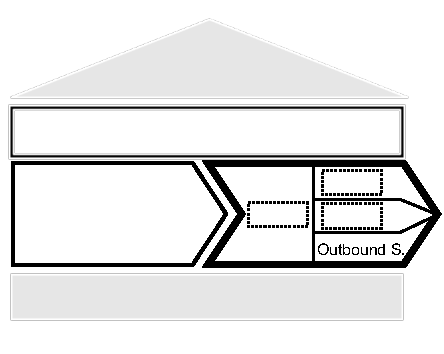
\includegraphics{figures/processes/outbound.pdf}
	 		\end{center}
	 	\end{subfigure}
	 	\begin{subfigure}[b]{.45\textwidth}
	 		\begin{center}
	 			\begin{tikzpicture}
	 			[node distance=.4cm, start chain=going below,font=\sffamily]
	 			\node[punktchain,rounded corners=0pt, join=by {-}] (eins)      {prepare contact};
	 			\node[punktchain,rounded corners=0pt, join=by {-}] (zwei) {contact customer};
	 			\node[punktchain,rounded corners=0pt, join=by {-}, ] (drei) {evaluate contact};
	 			\node[punktchain, draw=white ] (vier) { };
	 			
	 			\end{tikzpicture}
	 		\end{center}
	 	\end{subfigure}
	 	
	 \end{figure}
	 
	 A fundamental difference the \textsc{Inbound} and \textsc{Outbound} \textsc{Service} process is that outbound contact is proactive and needs more initial information to act on, whereas inbound contact is reactive \citep{DimensionData2015}. \Fig \ref{fig:outbound} shows the process, which is composed of three detail processes. Reflecting on the inbound process,  \textit{prepare contact} represents activities that take place prior to the activity that actually addresses the process object (route, preprocess, classify inquiry in \textsc{Inbound Service}). The following \textit{contact customer} step expresses the active approach of the customer (contact) from the company side and can mirror the process inquiry step in \textsc{Inbound Service}. Lastly, the \textit{evaluate contact} step contains subsequent efforts. Here the wording evaluate is chosen over review to put more focus on an assessment of the contact and less on the intention to change parts if necessary (\cf \ref{inb:review}). Furthermore, the company, as contact initiator, can perform a review at an earlier stage and does not need to react on a customer. 
	 
	 
	 \subsubsection{Prepare Contact}
	 
	 To actively approach a customer, there has to be a trigger or decision that lead to the initiation of the process, which is then assigned to the executing organizational unit, \eg, \acrshort{CSR}. The information that captures the intention behind the contact is assumed to be stored in the knowledge base. The first step of this detail process (\Fig \ref{fig:outbound:prep}) is consequently a query to get the \acrshort{CSR} informed, which is consistent over all channel variants. Next, the aforementioned reason for contact is processed by the \acrshort{CSR} to enable the transfer of it towards the upcoming contact of the customer. 
	 
	 All channels except voice show three blocks, that also appear in the review inquiry inbound process variant (draft, review, finalize message/post). This early (optional) verification by a supervisor is possible because the communication is started by the company and the purpose is stored in the known reason for contact. Therefore, there is no processing of a customer inquiry necessary on which a response is formulated. Because of this, direct messengers can also have these components, even though it is a synchronous channel. In the voice variant, there is no review. The \acrshort{CSR} is assumed to understand the reason for contact or resolve any issues with it in the \textit{process reason for contact} step, as the scripting of a call is implausible. 
	 
	 The case of a proactive post of a company on a customer's social profile might seem less typical on platforms like facebook, but it cannot be foreclosed. In addition, it depends on the social behavior on the network that might change over time and varies across networks.  
	 
	 \begin{figure}[caption={Prepare Contact Detail Process}, label={fig:outbound:prep}]
	 	
	 	\begin{subfigure}[b]{.45\textwidth}
	 		\centering
	 		\begin{tikzpicture}
	 		[node distance=.4cm,
	 		start chain=going below,font=\sffamily]
	 		
	 		\node[punktchain, join=by {-}] (eins)      {query knowledge base};
	 		\node[punktchain, join=by {-}] (zwei) {process reason for contact};
	 		\node[punktchain, join=by {-}] (drei) {draft message};
	 		\node[punktchain, join=by {-}] (vier) {review message};
	 		\node[punktchain, join=by {-}] (fuenf) {finalize message};
	 		
	 		\end{tikzpicture}
	 		
	 		\caption{Mail Variant}\label{fig:outbound:prep:mail}
	 	\end{subfigure}
	 	\begin{subfigure}[b]{.45\textwidth}
	 		\centering	
	 		\begin{tikzpicture}
	 		[node distance=.4cm,
	 		start chain=going below,font=\sffamily]
	 		
	 		\node[punktchain, join=by {-}] (eins)      {query knowledge base};
	 		\node[punktchain, join=by {-}] (zwei) {process reason for contact};
	 		\node[punktchain, join=by {-}] (drei) {draft post};
	 		\node[punktchain, join=by {-}] (vier) {review post};
	 		\node[punktchain, join=by {-}] (fuenf) {finalize post};
	 		\end{tikzpicture}
	 		\caption{Social Variant}\label{fig:outbound:prep:social}
	 	\end{subfigure}
	 	\begin{subfigure}[b]{.45\textwidth}
	 		\centering	
	 		\begin{tikzpicture}
	 		[node distance=.4cm,
	 		start chain=going below,font=\sffamily]
	 		\node[punktchain, draw=white] (null) { };
	 		\node[punktchain] (eins)      {query knowledge base};
	 		\node[punktchain, join=by {-}] (zwei) {process reason for contact};
	 		\node[punktchain, draw=white] (null) { };
	 		\node[punktchain, draw=white] (null) { };
	 		\node[punktchain, draw=white] (null) { };
	 		
	 		\end{tikzpicture}
	 		\caption{Voice Variant}\label{fig:outbound:prep:voice}
	 	\end{subfigure}
	 	\begin{subfigure}[b]{.45\textwidth}
	 		\centering	
	 		\begin{tikzpicture}
	 		[node distance=.4cm,
	 		start chain=going below,font=\sffamily]
	 		\node[punktchain, draw=white] (null) { };
	 		\node[punktchain] (eins) {query knowledge base};
	 		\node[punktchain, join=by {-}] (zwei) {process reason for contact};
	 		\node[punktchain, join=by {-}] (drei) {draft message};
	 		\node[punktchain, join=by {-}] (vier) {review message};
	 		\node[punktchain, join=by {-}] (fuenf) {finalize message};
	 		
	 		\end{tikzpicture}
	 		\caption{Direct Messenger Variant}\label{fig:outbound:prep:dm}
	 	\end{subfigure}
	 \end{figure}
	 
	 
	 \subsubsection{Contact Customer}
	 
	 The second step of \textsc{Outbound Service} models the approach of the client (\Fig \ref{fig:outbound:con}). The use of contact as a verb expresses that the customer is on the receiving end. (A)synchronous channels show a similar structure, respectively. As the message or post is already prepared, the select of the sending account and the actual transmission\footnote{Theoretically, the second block in the social variant should be named \textit{post post}. Considering writing style, the object is kept and the verb changed to send. } is left. As previously justified, the variant in social media includes a verification step of the network environment. 
	 
	 Synchronous communication establishes a \textit{conversation} with the customer on which is responded in a timely manner. It is noted that in contrast to the voice channel, a direct message does not require the customer to respond directly. With this open connection, the  \acrshort{CSR} is able to \textit{communicate} the \textit{reason of contact} to the customer. 
	 
	 As the contact is initiated by the company, the customer might not understand the reason for contact properly. In this case of synchronous communication, it is possible for the \acrshort{CSR} to\textit{ solve complications} on the spot. The last block of the contact customer detail process encompasses the \textit{solving} of \textit{further} \textit{questions}. Reason for this is that in the outbound case, there is object encapsulating the customer's need (as it is the inquiry in \textsc{Inbound Service}). Ergo, the customer can have additional unresolved questions which can, but not necessarily have to, relate to the reason of contact. In analogy to the \textit{solve inquiry} block in inbound processing, the verb solve is again used to emphasize the \acrshort{CSR}'s activity. 
	 
	 
	 \begin{figure}[caption={Contact Customer Detail Process}, label={fig:outbound:con}]
	 	
	 	\begin{subfigure}[b]{.45\textwidth}
	 		\centering
	 		\begin{tikzpicture}
	 		[node distance=.4cm,
	 		start chain=going below,font=\sffamily]
	 		
	 		\node[punktchain, join=by {-}] (eins)      {select account};
	 		\node[punktchain, join=by {-}] (zwei) {send message};
	 		\node[punktchain, draw=white] (null) { };
	 		\end{tikzpicture}
	 		
	 		\caption{Mail Variant}\label{fig:outbound:con:mail}
	 	\end{subfigure}
	 	\begin{subfigure}[b]{.45\textwidth}
	 		\centering	
	 		\begin{tikzpicture}
	 		[node distance=.4cm,
	 		start chain=going below,font=\sffamily]
	 		
	 		\node[punktchain, join=by {-}] (eins)      {select account};
	 		\node[punktchain, join=by {-}] (zwei) {verify environment};
	 		\node[punktchain, join=by {-}] (drei) {send post};
	 		\end{tikzpicture}
	 		\caption{Social Variant}\label{fig:outbound:con:social}
	 	\end{subfigure}
	 	\begin{subfigure}[b]{.45\textwidth}
	 		\centering	
	 		\begin{tikzpicture}
	 		[node distance=.4cm,
	 		start chain=going below,font=\sffamily]
	 		\node[punktchain, draw=white] (null) { };
	 		\node[punktchain] (eins)      {open conversation};
	 		\node[punktchain, join=by {-}] (zwei) {communicate reason for contact};
	 		\node[punktchain, join=by {-}] (drei) {solve complications};
	 		\node[punktchain, join=by {-}] (vier) {solve further questions};
	 		
	 		\end{tikzpicture}
	 		\caption{Voice Variant}\label{fig:outbound:con:voice}
	 	\end{subfigure}
	 	\begin{subfigure}[b]{.45\textwidth}
	 		\centering	
	 		\begin{tikzpicture}
	 		[node distance=.4cm,
	 		start chain=going below,font=\sffamily]
	 		\node[punktchain, draw=white] (null) { };
	 		\node[punktchain] (eins)      {open conversation};
	 		\node[punktchain, join=by {-}] (zwei) {communicate reason for contact};
	 		\node[punktchain, join=by {-}] (drei) {solve complications};
	 		\node[punktchain, join=by {-}] (vier) {solve further questions};
	 		
	 		\end{tikzpicture}
	 		\caption{Direct Messenger Variant}\label{fig:outbound:con:dm}
	 	\end{subfigure}
	 \end{figure}
	 
	 
	 
	 \subsubsection{Evaluate Contact}
	 
	 This detail process step (\Fig \ref{fig:outbound:eval}) closes the synchronous conversation and represents closing activities that are related to the contact. Synchronous channels close the conversation at the beginning, while asynchronous channels are completed with sending. Mirrored from the inbound process, the process building blocks \textit{update customer data} and \textit{update contact} draw a line to the review inquiry detail process. Here, the inquiry object is replaced by the contact object. 
	 
	 \begin{figure}[caption={Evaluate Contact Detail Process}, label={fig:outbound:eval}]
	 	
	 	\begin{subfigure}[b]{.45\textwidth}
	 		\centering
	 		\begin{tikzpicture}
	 		[node distance=.4cm,
	 		start chain=going below,font=\sffamily]
	 		
	 		\node[punktchain, join=by {-}] (eins)      {update customer data};
	 		\node[punktchain, join=by {-}] (zwei) {update contact};
	 		\end{tikzpicture}
	 		
	 		\caption{Mail Variant}\label{fig:outbound:eval:mail}
	 	\end{subfigure}
	 	\begin{subfigure}[b]{.45\textwidth}
	 		\centering	
	 		\begin{tikzpicture}
	 		[node distance=.4cm,
	 		start chain=going below,font=\sffamily]
	 		
	 		\node[punktchain, join=by {-}] (eins)      {update customer data};
	 		\node[punktchain, join=by {-}] (zwei) {update contact};
	 		\end{tikzpicture}
	 		\caption{Social Variant}\label{fig:outbound:eval:social}
	 	\end{subfigure}
	 	\begin{subfigure}[b]{.45\textwidth}
	 		\centering	
	 		\begin{tikzpicture}
	 		[node distance=.4cm,
	 		start chain=going below,font=\sffamily]
	 		\node[punktchain, draw=white] (null) { };
	 		\node[punktchain] (eins)      {close conversation};
	 		\node[punktchain, join=by {-}] (zwei) {update customer data};
	 		\node[punktchain, join=by {-}] (drei) {update contact};
	 		
	 		
	 		\end{tikzpicture}
	 		\caption{Voice Variant}\label{fig:outbound:eval:voice}
	 	\end{subfigure}
	 	\begin{subfigure}[b]{.45\textwidth}
	 		\centering	
	 		\begin{tikzpicture}
	 		[node distance=.4cm,
	 		start chain=going below,font=\sffamily]
	 		\node[punktchain, draw=white] (null) { };
	 		\node[punktchain] (eins)      {close conversation};
	 		\node[punktchain, join=by {-}] (zwei) {update customer data};
	 		\node[punktchain, join=by {-}] (drei) {update contact};
	 		
	 		\end{tikzpicture}
	 		\caption{Direct Messenger Variant}\label{fig:outbound:eval:dm}
	 	\end{subfigure}
	 \end{figure}
	 
	 	\subsection{Self-Service}
	 	 \label{pr:sel}
	 The third customer interaction process is not subject to inter-personal service \citep{Thomas2008self} and focuses on ways that enable the customer to be the main value-generating part in the service interaction. This is facilitated by a technological component which can relieve the customer of a varying extent of the problem. The following illustrates this continuum from a customer perspective: Simple self-services, like an \acrshort{FAQ} section offer answers to questions, which the customer has to select from a list. The customer must express the need, map it to available information, select the appropriate answer and process its content. A more advanced self-service might be able to additionally support the customer at expression of the need and takes care of mapping through a textual input, which is a more natural way of communication. The textual input is analyzed and algorithmically mapped to the most appropriate resolution\footnote{A \textit{solution} is used in context of the provider's service products, which is why resolution is taken here.}, which is then presented to the customer, who must consume its content and is hopefully satisfied. It is noted that both resolution address the customer's issue, but sophisticated \acrshort{IT} increases usability by an easier interface to the customer's issue and a computed provision of a resolution. This addresses what \cite{Thomas2008self} names a minimal skill set, \viz an increased usability decreases the minimal skill set that is required for use. 
	 
	 From literature \citep{meuter2000self, Thomas2008self, Thomas:2009}, one can identify characteristics of self-services, which need to be considered in a process. As the provider's perspective is shown, the process needs to hold aspects which are seen from a system perspective. The previous example features the differences between simple and technological enhanced serf-services. In both cases, the system has to provide information, but simple self-services require the capability to express the need in the language of the service system, while the second allowes the customer to express it in natural language. The system perspective implies that the more active the customer takes the part in the process (\ie the simpler the self-service is), the less parts of the process are carried out by the system. 
	 
	 Furthermore, a self-service can be seen as part of another customer service process. One can think it as support for a inter-personal contact, when it provides resolutions based on customer information. Examples for this are \acrshort{IVR} or generated chat messages based on customer input.
	 
	 Unlike inter-personal services, self-services cannot be structured \wrt a communication channel, as they can be part of a service within one or multiple channels, or stand-alone in a web-based setting. A process representation is chosen which models both a supporting self-service and a stand-alone implementation.
	 
	 \begin{figure}[caption={\textsc{Self-Service} Process}, label={fig:selfservice}]
	 	\begin{subfigure}[b]{.45\textwidth}
	 		\begin{center}
	 			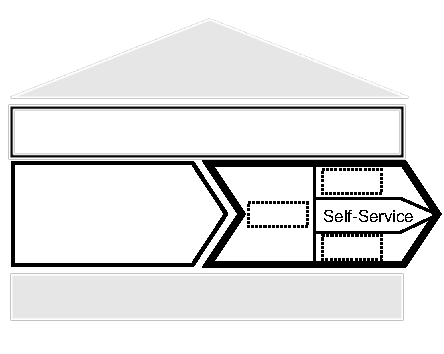
\includegraphics{figures/processes/selfservice.pdf}
	 		\end{center}
	 	\end{subfigure}
	 	\begin{subfigure}[b]{.45\textwidth}
	 		\begin{center}
	 			\begin{tikzpicture}
	 			[node distance=.4cm, start chain=going below,font=\sffamily]
	 			\node[punktchain, rounded corners = 0pt, join=by {-}] (eins)      {identify customer needs};
	 			\node[punktchain,  rounded corners = 0pt,  join=by {-}] (zwei) {process customer needs};
	 			\node[punktchain,  rounded corners = 0pt, join=by {-}, ] (drei) {present resolution};
	 			\node[punktchain, rounded corners = 0pt,  join=by {-}, ] (vier) {evaluate resolution};
	 			
	 			\end{tikzpicture}
	 		\end{center}
	 	\end{subfigure}
	 	
	 \end{figure}
	 
	 The process object \textit{customer need} is chosen over inquiry. It is noted that a customer need is an abstract construct that is used to express the customer's intention of use. However, like the inbound process self-service gets input from a customer and tries to solve the issue. But as there is no \acrshort{CSR} directly involved, there is less certainty that the system adequately addresses the \enquote{inquiry}. Due to this lack of a human counterpart on provider side, the technological interface provided by the system to the customer takes an important part in \textit{identifying customer needs}. As the capabilities of this interface vary drastically among different self-service scenarios, customer needs are chosen to emphasize the difference to inbound processing. \textit{Process customer needs} then aims at mapping the identified need to a defined resolution in the knowledge base. After creation, \textit{present resolution} communicates the findings to the customer. Lastly, \textit{evaluate resolution} represents post-processing activities. The process is shown in \Fig \ref{fig:selfservice}.
	 
	 The building blocks of the four detail processes are summarized in \Fig \ref{fig:selfservice:detail}, as their is no further split into variants. The following description emphasizes the differences in simple and advanced self-service scenarios. 
	 
	 \subsubsection{Identify Customer Needs}
	 The building blocks of \textit{identfiy customer needs} (\Fig \ref{fig:selfservice:1}) capture external circumstances, that might be processed by the system to have more data available for inferring the customer need. Environmental factors are implicitly collected, \ie the customer does not need to state them. \textit{Request information} models the input that the customer gives to the system. While active phrasing might fit to more advanced self-service systems better than to simple \acrshort{FAQ}s (as the latter hardly asks the customer for information), the step applies to the concept of self-services: in order to narrow down the customer needs, relevant information needs to be selected by the customer (in a simple self-service system) or demanded as input for the system (in the advanced case). The verb \textit{infer} is used to describe the stochastic component of the system's attempt to understand the customer need. Again, the selection of a \acrshort{FAQ} entry by the customer might minimize the system's influence, still it conceives the selection as an information input and infers that the customer is \textit{needing} answers in this regard. An increased usability in the technological interface (arbitrary text input instead of a selection of options) also increases uncertainty in need identification, because the system has to select the fitting case by itself. 
	 \subsubsection{Process Customer Needs}
	 After the customer needs are inferred and hence available in a manner that corresponds to the data available in the knowledge base, the \textit{process customer needs} detail process (\Fig \ref{fig:selfservice:2}) receives suitable information and creates a resolution that represents the appropriate response to the customer's need. This can be needed information, so that the need is completely addressed. Another option is that the self-service system can identify the need, but solving it requires personal-interaction. This expresses the limitations of service automation. 
	 
	 \subsubsection{Present Solution}
	 \textit{Present resolution} (\Fig \ref{fig:selfservice:3}) conveys the result to the customer. The resolution is presented by the system in response to the customer's input. The customer's reaction is an important indicator of satisfaction and captured during the presentation. As the identification of a customer is not required for self-service use, these data needs to be stored in relation to the self-service input to further improve customer experience. 
	 
	 \subsubsection{Evaluate Solution}
	 The last detail process \textit{evaluate resolution} (\Fig \ref{fig:selfservice:4}) can include a request for feedback (\textit{Did this solve your problem?}) and finally all relevant information is stored and hence updates knowledge base, similar to \textsc{Inbound} and \textsc{Outbound Services}.
	 
	 \begin{figure}[caption={\textsc{Self-Service} Detail Processes}, label={fig:selfservice:detail}]
	 	
	 	\begin{subfigure}[b]{.45\textwidth}
	 		\centering
	 		\begin{tikzpicture}
	 		[node distance=.4cm,
	 		start chain=going below,font=\sffamily]
	 		
	 		\node[punktchain, join=by {-}] (eins)      {analyze environment};
	 		\node[punktchain, join=by {-}] (zwei)      {request information};
	 		\node[punktchain, join=by {-}] (eins)      {infer customer needs};
	 		
	 		
	 		\end{tikzpicture}
	 		
	 		\caption{Identify Customer Needs}\label{fig:selfservice:1}
	 	\end{subfigure}
	 	\begin{subfigure}[b]{.45\textwidth}
	 		\centering	
	 		\begin{tikzpicture}
	 		[node distance=.4cm,
	 		start chain=going below,font=\sffamily]
	 		
	 		\node[punktchain, join=by {-}] (zwei) {query knowledge base};
	 		%	\node[punktchain, join=by {-}] (zwei) {integrate subsystem information};
	 		\node[punktchain, join=by {-}] (drei) {create resolution};
	 		\node[punktchain, draw=white,text=white] (sechs) {verify environment};
	 		\end{tikzpicture}
	 		\caption{Process Customer Needs}\label{fig:selfservice:2}
	 	\end{subfigure}
	 	\begin{subfigure}[b]{.45\textwidth}
	 		\centering	
	 		\begin{tikzpicture}
	 		[node distance=.4cm,
	 		start chain=going below,font=\sffamily]
	 		\node[punktchain, draw=white] (null) { };
	 		\node[punktchain] (eins)      {present resolution};
	 		\node[punktchain, join=by {-}] (zwei) {process customer reaction};
	 		\end{tikzpicture}
	 		\caption{Present Resolution}\label{fig:selfservice:3}
	 	\end{subfigure}
	 	\begin{subfigure}[b]{.45\textwidth}
	 		\centering	
	 		\begin{tikzpicture}
	 		[node distance=.4cm,
	 		start chain=going below,font=\sffamily]
	 		\node[punktchain, draw=white] (null) { };
	 		\node[punktchain] (eins) {request feedback};
	 		\node[punktchain, join=by {-}] (zwei) {update knowledge base};
	 		
	 		\end{tikzpicture}
	 		\caption{Evaluate Resolution}\label{fig:selfservice:4}
	 	\end{subfigure}
	 \end{figure}
	 
	 
	 \subsection{Knowledge Management}
	 \label{pr:kno}

Knowledge management is a widely used term across different fields of academic research. \cite{girard2015defining} compile over 100 definitions and analyze their content. They propose to define it as \enquote{the process of creating, sharing, using and managing the knowledge and information used in an organization\footnote{Organization refers to a client business in this case.}}\citep[\p{14}]{girard2015defining}. It is noted that this definition can be criticized as too general, but chosen because it takes a process view and fits to the position in the framework: The interpretation as part of customer-facing processes emphasizes the role of \textsc{Knowledge Management} in operational business. Hence, this view on knowledge management limits its boundaries to a certain client business. Knowledge management for the provider organization is seen as an important aspect, yet it encompasses various areas which are separated into distinct management processes. Therefore it is desisted from the creation of an additional global knowledge management process. The importance of knowledge management in operations is stressed by its third rank regarding upcoming investments in contact centers \citep{ccnet2016}. 

Building on the previously proposed \acrshort{ERM} for customer-facing services (\Fig \ref{fig:contacterm}), a transaction, customer and case are entities that stand in relation to the customer contact. The latter represents the business object of the three services that form the interface to the customer. In these processes, the remaining transaction, customer and case entity become an integral component and shall be modeled as three variants of the main process \textsc{Knowlege Management}.

\acrshort{CSR}s need a source of information so that they can adequately perform the mapping of customer inquiries to organizational knowledge. When the cancellation of contract is requested by a customer, the \acrshort{CSR} can look up whether a case exists that contains the knowledge to satisfy the customer, \viz instructions for performing the cancellation in relevant systems. In a self-service scenario, the knowledge base is largely defining the capabilities of the service. 

Transactions capture events and are always connected to a customer. They relate to a product or a touch point and have a hierarchy: a purchase can be the result of a previous touch point (informing about product features for instance). This information is 	indispensable to uncover a customer journey and the more transactions are known, the better the \acrshort{CSR}'s understanding of the customer can be. 

The customer as the focal point in \acrshort{CRM} and may or may not be known during a contact. When an identification can be performed, the knowledge base provides information regarding master data and transactions assigned to the entity. In order to achieve an omni-channel \acrshort{CRM} experience, the existence of a knowledge base about customers is critical for providing personalized services. 

Myriad frameworks try to distillate the essence of knowledge management. \cite{Rubenstein_Montano_2001} have examined various proposals and compared their similarities. Drawing on their analysis, activities in these frameworks serve as basis for the assessment of their applicability in the reference model. The omission of strategic frameworks narrows down the list. Frameworks that do not contain a procedural description are also excluded from further consideration. As several of the remaining frameworks show rather abstract and philosophical characteristics, the ones showing activities that can be understood from an \acrshort{IS} perspective are selected. After evaluating the remaining four frameworks (\cf Appendix \ref{app:knowmang}), the work of \cite{van_Heijst_1997} is chosen as a basis.

Listed basic processes in the work of \citeauthor{van_Heijst_1997} are knowledge development (1), combination (2), consolidation (3) and distribution (4). They refer to the knowledge cycle in \citep{Wiig_1997}, where these are constituents of the \textit{act}-phases\footnote{The cycle contains four phases in total: conceptualize, reflect, act, review}. This placement fits well into the operational interpretation that resides in the reference model's \textsc{Knowledge Management} process.

Development is seen here as the acquisition of new knowledge  \citep{van_Heijst_1997} and the maintenance of the knowledge base. Combination uses the connection of different knowledge sources as a lever, which especially gets important in the field of omni-channel \acrshort{CRM}. Consolidating signifies the processing of knowledge data so that it is available and usable. This relates on the one hand to analytical activities so that decisions can be based on aggregated data (\eg, classification in self-services). On the other hand, indexing and structuring of knowledge is necessary to facilitate fast access. This is important in manual access through \acrshort{CSR}s, as well as in the case of a self-service technology. Lastly, the distribution of knowledge describes the provision of knowledge to the organization. As the customer-facing processes show \textit{query knowledge base} as the active part of requesting, its counterpart is seen in this last process of \textsc{Knowledge Management}. 

In order to fit the three variants (case-related, customer-related, transaction-related) to these steps, the verbs \textit{maintain}, \textit{consolidate}, \textit{combine} and \textit{provide} are used to represent the four detail processes. The object in the main process variants corresponds to the information that stands in center of the variant(\eg, case data, customer data, transaction data), which reasons the split so that distinct process building blocks can be added. 
%disclaimer
For this thesis, only the textual description of the processes shall represent their content. There is no explicit modeling of the lowest layer of the framework. 

\begin{figure}[caption={\textsc{Knowledge Management} Main Process Variants}, label={fig:knowledge}]
	\begin{subfigure}[b]{.6\textwidth}
		\begin{center}
			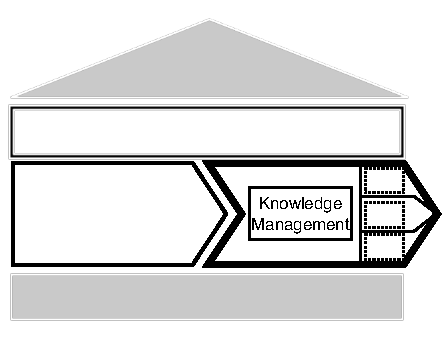
\includegraphics{figures/processes/knowledgemanagement.pdf}
		\end{center}
	\end{subfigure}

	\begin{subfigure}[b]{.32\textwidth}
		\begin{center}
			\begin{tikzpicture}
			[node distance=.4cm, minimum height=4.5em, start chain=going below,font=\sffamily]
			\node[punktchain, rounded corners=0pt , minimum height=2.8em,join=by {-}] (eins)      {maintain case master data};
			\node[punktchain,rounded corners=0pt, minimum height=2.8em,  join=by {-}] (zwei) {consolidate case data };
			\node[punktchain, rounded corners=0pt, minimum height=2.8em, join=by {-}, ] (drei) {combine case data};
			\node[punktchain, rounded corners=0pt, minimum height=2.8em, join=by {-}, ] (vier) {provide case data };

			\end{tikzpicture}
			\caption{Case-related Variant}\label{fig:knowmang:case}
		\end{center}
	\end{subfigure}
\begin{subfigure}[b]{.32\textwidth}
	\begin{center}
		\begin{tikzpicture}
		[node distance=.4cm, start chain=going below,font=\sffamily]
		\node[punktchain, rounded corners=0pt, minimum height=2.8em,join=by {-}] (eins)      {maintain customer master data};
		\node[punktchain,rounded corners=0pt,  
		minimum height=2.8em,join=by {-}] (zwei) {consolidate customer data};
		\node[punktchain, rounded corners=0pt,  
		 minimum height=2.8em,join=by {-}, ] (drei) {combine customer data};
		\node[punktchain, minimum height=2.8em, rounded corners=0pt, join=by {-}, ] (vier) {provide customer data};
	
		\end{tikzpicture}
				\caption{Customer-related Variant}\label{fig:knowmang:cust}
	\end{center}
\end{subfigure}
\begin{subfigure}[b]{.32\textwidth}
	\begin{center}
		\begin{tikzpicture}
		[node distance=.4cm, start chain=going below,font=\sffamily]
		\node[punktchain, rounded corners=0pt,minimum height=2.8em ,join=by {-}] (eins)      {maintain transaction data};
		\node[punktchain,rounded corners=0pt, minimum height=2.8em , join=by {-}] (zwei) {consolidate transaction data};
		\node[punktchain, rounded corners=0pt, minimum height=2.8em, join=by {-}, ] (drei) {combine transaction data};
		\node[punktchain, rounded corners=0pt , minimum height=2.8em,join=by {-}, ] (vier) {provide transaction data};
		
		\end{tikzpicture}
				\caption{Transaction-related Variant}\label{fig:knowmang:trans}
	\end{center}
\end{subfigure}
	
\end{figure}
	 
	%%%%%%%%%%
	
	
	

	
	
	
	
	% klar definieren was ich unter sst verstehe \citep{Thomas:2009} hält auch online tech support boards, live chat sessions with customer support personal, user forums, etc. drin. also da wo der CSR noch supported. 
	%starting point \citep{Thomas:2009}.
	%When a customer calls into the call center for technical support, it is often with the belief that they are contacting a CSR who is either an expert at solving their problem or at least more knowledgeable about their problem than the caller.
	%	 \citep{ccn2016} s.44
	
	%	To determine the most efficient, effective and mutually acceptable use of technology in service delivery, the customer's perspective needs to be known and understood.  \citep{Walker_2002}
	\newpage
	
	
	
	
	\section{Client Processes}
	With the process structure being discussed in \ref{sec:srproc}, the following processes are described \wrt the outsourcing lifecycle: \textsc{Sales}, leading to \textsc{Transition} followed by \textsc{Account Management}. \textsc{Solution Design} is specified at last to emphasize its connection to the following management processes. Underlying process building blocks of client processes are not explicitly specified in this work, but suggestions for components are given in the textually. 
	
	In relation to the other two process groups of the framework, the client processes show the smallest \acrshort{BPO} domain specificity, as the outsourcing process and agreement between provider and client stands in focus. \acrshort{CRM} encloses the services themselves, but it does not impact the B2B-relationship that forms around provider and client in order to establish the service transition. 
	
	It is common practice that a company interested in outsourcing first issues a \acrfull{RFI} to inform providers about its plans and to receive information about their willingness to participate in a bid. A following \acrfull{RFP} considers a smaller group of provider's to narrow down candidates and is asking for a more detailed offer. As the relationship between both parties gets concrete, the here described processes take action. 
	
	\subsection{Sales}
	\label{pr:sal}
	This process marks the starting point of an outsourcing lifecycle of a provider with a client. Building on a review existing paradigms for B2B-selling processes in the literature \citep{_ge_2011}, a linear process known as the  \enquote{seven steps of selling} shall serve as a blueprint for the process structure. 
	
	With roots in the 1920s, \cite{Moncrief_2005} review the traditional seven steps and focus on its applicability towards relationship selling, which aims at the \enquote{securing, building, and maintaining long-term relationships with profitable customers\footnote{ Clients are meant the outsourcing terminology.}} \citep[\p{13}]{Moncrief_2005}. The technological progress has impacted the steps significantly, which is why the wording is to be accepted with reservation. The steps are Prospecting (1), Preapproach (2), Approach (3), Presentation (4), Overcoming Objections (5), Close (6), Follow-Up (7). In contrast to the initial intent, the steps do not need to be sequentially completed and multiple people are involved instead of a single sales person. Moreover, it is abstracted from the physical meaning of \textit{approach} or \textit{presentation} for instance.
	
	\Fig \ref{fig:salesproc} shows the \textsc{Sales} process and its detail processes are discussed in the following \wrt the seven steps of selling. 
	
	\begin{figure}[caption={\textsc{Sales} Process}, label={fig:salesproc}]
		\begin{subfigure}[b]{.40\textwidth}
			\begin{center}
				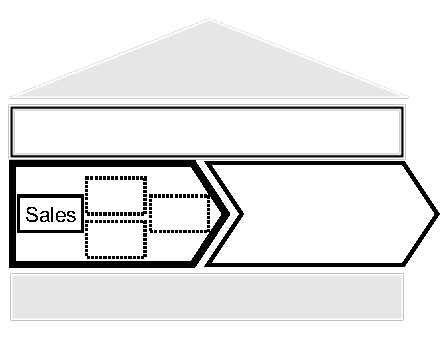
\includegraphics{figures/processes/sales.pdf}
			\end{center}
		\end{subfigure}
		\begin{subfigure}[b]{.9\textwidth}
			\begin{center}
				\begin{tikzpicture}
				[node distance=.4cm, start chain=going below,font=\sffamily]
				\node[punktchain, rounded corners=0pt, join=by {-}] (eins)      {identify prospect};
				\node[punktchain, rounded corners=0pt, join=by {-}] (zwei) {approach prospect};
				\node[punktchain, rounded corners=0pt, join=by {-}, ] (drei) {evaluate \acrshort{RFP}};
				\node[punktchain, rounded corners=0pt, join=by {-}, ] (vier) {create offer};
				\node[punktchain, rounded corners = 0pt,] (fuenf) {negotiate contract};
				\node[punktchain, left = of fuenf, rounded corners = 0pt,] (sechs) {perform due diligence};
				\node[punktchain, right = of fuenf, rounded corners = 0pt,] (sieben) {create commercial deal};
				\node[punktchain, below = of fuenf, rounded corners = 0pt,] (acht) {create contract};
				\draw[|-,-|,-, thick,] (vier.south) |-+(0,-0.5em)-| (fuenf.north);
				\draw[|-,-|,-, thick,] (vier.south) |-+(0,-0.5em)-| (sechs.north);
				\draw[|-,-|,-, thick,] (vier.south) |-+(0,-0.5em)-| (sieben.north);
				\draw[|-,-|,-, thick,] (fuenf.south) |-+(0,-0.5em)-| (acht.north);
				\draw[|-,-|,-, thick,] (sechs.south) |-+(0,-0.5em)-| (acht.north);
				\draw[|-,-|,-, thick,] (sieben.south) |-+(0,-0.5em)-| (acht.north);
				\end{tikzpicture}
			\end{center}
		\end{subfigure}
		
	\end{figure}
	
	\subsubsection{Identify Prospects}
	In order to enable a pro-active client approach in the selling process, the market has to be analyzed so that potential clients can be targeted by the provider. It corresponds to the first step of selling (Prospecting), while the efforts towards a specific prospect can be seen as part of \textit{Preapproach}. 
	A prospect can be \enquote{ regarded [...] as a potential customer, client, \etc} \citep{oxfordprospect} and the provider's perception is that this organization can benefit from outsourcing processes. This activity requires the screening of in-house services, so that added-value can be worked out. As there is no internal information (for example about costs) available at this point, this detail process is especially important in scenarios where the \acrshort{BPO} provider sees its strengths in providing a better service over solely cost reduction. The prospect might not be aware of the efforts of the provider and might not consider outsourcing as an option. Hence, the provider can expand its market and bring itself in an advantageous position in the following contact with the client. 
	
	
	\subsubsection{Approach Prospects}
	
	Building on the market analysis that brings out a prospect, this step describes the provider's \textit{Approach} towards the potential client, so that the provider can communicate its ideas. Clearly, this describes the third step of selling. The prospect can evaluate these ideas and form a clearer picture of the circumstances, as these must base on assumptions due to lack of internal information. In the positive case, the prospect creates a bid, which represents the prospect's intent to engage in outsourcing of a specified process. Considered providers are contacted and receive an \acrshort{RFP}\footnote{Technically, the \acrshort{RFI} is issued beforehand. However, from a process perspective it is seen as similar an \acrshort{RFP}, yet it comprises less detail. To avoid redundancy and emphasize the importance of a \acrshort{RFP} \wrt a \acrshort{RFI}, only the former is explicitly modeled.}.
	
	The hitherto described two detail processes of selling can be seen as optional. If a client contacts a provider self-motivated, the process starts with evaluation of the \acrshort{RFP}.  
	
	\subsubsection{Evaluate \acrshort{RFP}}
	
	The third detail process has no direct reference to selling process, but is important  from the provider's perspective.  This is due to the fact that in the selling process, the willingness of the selling party is not in question. However, in the domain of outsourcing, a matching between client needs and offered services by the provider is necessary. Furthermore, the action of issuing the \acrshort{RFP} (initiated by the prospect) requires a \textit{reaction} of the provider. This reaction needs to consider the requirements of the prospect internally in order to decide whether to participate in the bid. This evaluation examines the fit to the provider's service offerings, its sales strategy, but also macro-environmental factors of the bid. The PEST-framework \citep{0314852336} illustrates these as a mnemonic for political, economic, social and technological aspects that surround and influence the decision of a provider. 
	When the provider decides to continue the sales activity, the following process step, namely the creation of an offer is initiated. 
	
	\subsubsection{Create Offer}
	The fourth detail process describes the activities that are done to respond  to the client's \acrshort{RFP} by means of an offer. The corresponding fourth step in the selling (Presentation), is described as the demonstration of the seller's products in terms of features, advantages and benefits \citep{Moncrief_2005}. This can also be implicitly seen in the offer, only that the boundaries are given by the \acrshort{RFP}. However, providers need to make assumptions in the process. 
	
	As multiple providers receive an \acrshort{RFP}, there is competition. It is common for \acrshort{RFP} issuing companies to narrow down the candidates by creation of a \textit{short list} after reviewing responses. This short list marks the next stage in the provider selection process, where more details are given to the remaining providers. In turn, these work in new information to further specify the offer. The final selection of a provider is a decision by the prospect, which is why it is not further modeled in this process. 
	
	The following fifth part of \textsc{Sales} is split into three parts in order to emphasize their connection to the fifth part of the steps of selling (overcoming objections). 
	
	
	\subsubsection{Negotiate Contract}
	
	As the client\footnote{The contract describes a state where both parties have agreed to do outsourcing. Therefore, the term client is used instead of prospect from now on.} and provider move closer to an outsourcing agreement, both need to discuss terms and conditions. To capture mutual understanding, documents like a \acrfull{LOI} or a \acrfull{MOU} can be established. The contract is the legal formalization of the relationship between provider and the client \citep{Franceschini_2003}.
	
	Covered aspects can be the operating model, process and scope, technology and tools, people, change management, transition planning, location management, security \& control, regulation or data privacy for instance \citep{deloittehandbook}. 
	Of special importance is the \acrfull{SLA}, that describes \enquote{the performance level at which the service should be provided by the client} \citep[\p{32}]{deloittehandbook}. The contract specifies these to align the operational objectives of both parties and to incentivize correct behavior. Related to \acrshort{SLA}s is a credits regime, which specifies how performance below the \acrshort{SLA} is treated. 
	
	Aim of this detail process is to find an agreement, so that both parties are willing to set up and sign the contract.
	
	\subsubsection{Perform Due Diligence}
	
	Outsourcing can involve the transfer of personnel, hardware, software, contracts or licensing agreements. The decrease of information asymmetries between client and prospect helps the provider to compile a more detailed offer. Goal of due diligence is the systematic determination of all contents and related processes with respect to the outsourced services, so that there is a foundation to assess the project and its measures \citep[\p{13}]{bitkom2008}. This act of collecting knowledge minimizes risk by depending less on assumptions and hence aims at including more information from the client side in \textsc{sales}. 
	
	\subsubsection{Create Commercial Deal}
	
	The provider needs to develop a commercial model for its services that are subject to this outsourcing project. Financial engineering of the provider leads to a pricing model that needs to be agreed on\footnote{This agreement is reason for naming the object commercial deal instead of commercial model.}. The reader is referred to Appendix \ref{app:fineng} for typical pricing model elements. The activity of defining a commercial model is \textit{provider-oriented}, which is reason for its explicit modeling \wrt \textit{client-oriented} due diligence and \textit{bilateral} negotiation detail process. 
	
	\subsubsection{Create Contract}
	
	The sixth step of selling (close) describes the agreement of selling and buying party. In \acrshort{BPO} this document is represented by multiple contracts between provider and client. Previous negotiations, information from due diligence and the commercial deal are foundations for setup of contracts. This detail process ends with the signing of the documents, which leads to the transition phase of the outsourcing lifecycle. Usually there are separate contracts for outsourcing and the transition project \citep{bitkom2008}. 
	
	The seventh step of selling (follow-up) is represented in the \textsc{Account Management} process that covers the development of an existing outsourcing relationship. 
	
	
	\subsection{Transition}
		 \label{pr:tra}
	The objective of this process is to set the outsourcing into place by transition of work and resources. Transition\footnote{\enquote{The process or a period of changing from one state or condition to another.} \citep{oxfordtransition}} and transformation\footnote{\enquote{A marked change in form, nature, or appearance.} \citep{oxfordtransformation}} are two dominant terms for this phase. The former seems to have more popularity in literature \citep{perunovic2007outsourcing}, as its defining change aspect underlines the shift from the client to the provider. 
	
	The process, shown in \Fig \ref{fig:transproc}, is built around the transition plan object, which captures important steps during the transition project. It is noted that this plan needs to be conceptualized during contract negotiations and before signing the agreement, however \cite{deloittehandbook} lists \textit{develop transition plan} as part of the transition phase. This intersection of \textsc{sales} and \textsc{transition} reasons their separation. The responsibility for the business is given to the provider in the \textit{transfer business} detail process, followed by knowledge transfer in the three dimensions people, process and technology. 
	
	Three phases can be identified during the project \citep{bitkom2008, 0273705601}. In the \acrfull{PMO} phase the business is continued in an as-is state, while the following  \acrfull{TMO} phase implements changes. The objective is to reach \acrfull{FMO}, that fulfills the requirements of the to-be state. However, this last phase is not part of the transition process, but normal operations. 
	
	\begin{figure}[caption={\textsc{Transition} Process}, label={fig:transproc}]
		\begin{subfigure}[b]{.40\textwidth}
			\begin{center}
				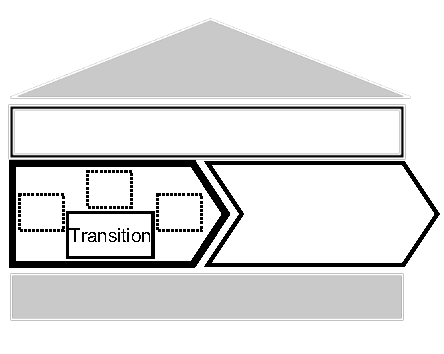
\includegraphics{figures/processes/transition.pdf}
			\end{center}
		\end{subfigure}
		\begin{subfigure}[b]{.9\textwidth}
			\begin{center}
				\begin{tikzpicture}
				[node distance=.4cm, start chain=going below,font=\sffamily]
				\node[punktchain, rounded corners=0pt, join=by {-}] (eins)      {develop transition plan};
				
				
				\node[punktchain, rounded corners=0pt, join=by {-}, ] (vier) {transfer business};
				\node[punktchain, rounded corners = 0pt,] (fuenf) {transfer process};
				\node[punktchain, left = of fuenf, rounded corners = 0pt,] (sechs) {transfer people};
				\node[punktchain, right = of fuenf,  rounded corners = 0pt,] (sieben) {transfer technology};
				\node[punktchain, below = of fuenf, rounded corners = 0pt,] (acht) {perform PMO phase};
				\node[punktchain, rounded corners = 0pt,join=by {-}, ] (neun) {perform TMO phase};
				\draw[|-,-|,-, thick,] (vier.south) |-+(0,-0.5em)-| (fuenf.north);
				\draw[|-,-|,-, thick,] (vier.south) |-+(0,-0.5em)-| (sechs.north);
				\draw[|-,-|,-, thick,] (vier.south) |-+(0,-0.5em)-| (sieben.north);
				\draw[|-,-|,-, thick,] (fuenf.south) |-+(0,-0.5em)-| (acht.north);
				\draw[|-,-|,-, thick,] (sechs.south) |-+(0,-0.5em)-| (acht.north);
				\draw[|-,-|,-, thick,] (sieben.south) |-+(0,-0.5em)-| (acht.north);
				\end{tikzpicture}
			\end{center}
		\end{subfigure}
		
	\end{figure}
	
	\subsubsection{Develop Transition Plan}
	Provider and client collaboratively develop a transition plan, that shows similarities to a project plan. A schedule, milestones and a work breakdown structure help to prepare both parties for the upcoming transition. Stakeholder commitment is important and a governance concept needs to be established for ensuring a frictionless course of action \citep{itgov2005}. The planning of work and especially knowledge transfer is another important aspect and linked to the project's success \citep{deloittehandbook}. 
	
	The completion of the transition plan marks the end of this detail process. While this step can start before completion of \textsc{sales}, the following activities represent the contract's execution and are consequently realized after an agreement of both parties. There is no explicit \textit{implement transition plan} detail process, because all of the following detail processes can be subsumed under this wording and thereby make it hardly expressive. 
	
	\subsubsection{Transfer Business}
	
	The transfer of the business has the objective to bring the provider into control. One can also argue that this detail process must take place after underlying components (\ie people, process, technology) are transferred, so that details are specified before the provider is in charge. Another position can be that in order to orchestrate the components, knowledge about the entire business needs to be achieved. This perspective is preferred here and is reason for naming it the \textit{objective} of the detail process to take over control, so that knowledge transfer can take place before the responsibilities change. 
	
	Knowledge transfer is an important aspect and implicitly included in this and the following detail processes. A separate knowledge transfer detail process is not modeled, because it is seen as too unspecific for the transition step. Instead, the use of the verb \textit{transfer} shall emphasize its importance across the different dimensions. 
	
	The shift of the business to the outsourcing provider has to mind legal admissibility\footnote{In German law \cf §613a BGB. }, that especially has implications on the transfer of staff. Moreover, the acquisition of tangible assets is to be handled. 
	
	\subsubsection{Transfer People, Process, Technology}
	
	Building on the people, process, technology split discussed in context of  \acrshort{BPO} in \acrshort{CRM} (\cf \ref{sec:proide}), each detail process emphasizes the respective aspect. In addition to knowledge transfer that enables the provider to know \textit{how} the client organization has worked in the past \citep{perunovic2007outsourcing}, the provider has to integrate its own resources that enable an improvement over status-quo.
	
	 Training of existing staff towards new tasks or training of new personnel can be named in the \textit{people} dimension. The \textit{transfer process} step sets up new processes that are part of the service delivery. Lastly, \textit{technology transfer} establishes the compatibility of existing and new systems for service delivery. The provider's solution is influencing at this point. While the design of the solution is located in a separate process, its outcome is integrated in this part of \textsc{transition}. 
	
	\subsubsection{Perform \acrshort{PMO} Phase}
	\todo{neu machen}The \acrshort{PMO}\footnote{Current Mode of Operation (CMO) is used synonymously. } phase starts with the transit of resources and responsibilities \citep{bitkom2008}. Its aim is to stabilize the business after shifting it to the provider. With respect to the transition plan, its duration is limited so that intended changes can be performed shortly after in the \acrshort{TMO} phase.
	
	\subsubsection{Perform \acrshort{TMO} Phase}
	After the as-is state is operating under the provider's responsibility, the implementation of changes can be initiated. The complexity of changes depend on the degree of innovation in the provided services \wrt as-is services. Reaching the \acrshort{FMO} phase ends this phase. With the service solutions in place, the regular \acrshort{SLA} and credit regime applies.
	
	
	%Deloitte: differentiate between service definition (\ie requirements) and service solution (how provider meets the requirements)
	
	
	%hier service architecture, product, configuration kurz erklären und %nur auf die konfiguration eingehen. sagen, dass es auf product aus portfolio basiert, welches dann für client reqs angepasst werden muss. das ist dann der theorieteil, worum man den prozess baut. 
	
	
	
	\subsection{Account Management}
		 \label{pr:acc}
	An account can be defined as \enquote{a contract to do work for a client} \citep{oxfordaccount}. To emphasize its relation to an existing business, this notion is chosen over other wordings in outsourcing frameworks like \textit{outsourcing management} \citep{Franceschini_2003} or \textit{managing relationship} \citep{perunovic2007outsourcing}. In essence, it frames the relationship between provider and client after an outsourcing agreement is established. Consequently, it has elements of \acrshort{CRM} with the client as subject. Taking a strategic perspective (\cf \ref{sec:crm}), this process aims at maximizing (client) value and corporate profitability \citep{payne2004role}. An account is the corresponding business object to the process. \cite{reinartz2004customer} name relationship initiation, maintenance and termination as temporal stages in the \acrshort{CRM} process, which is used for structuring \textsc{Account Management} (\Fig \ref{fig:amproc}).
	
	\begin{figure}[caption={\textsc{Account Management} Process}, label={fig:amproc}]
		\begin{subfigure}[c]{.45\textwidth}
			\begin{center}
				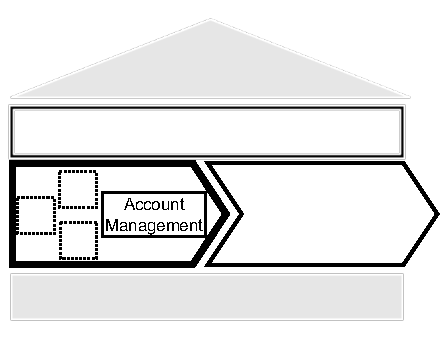
\includegraphics{figures/processes/accountmanagement.pdf}
			\end{center}
		\end{subfigure}
		\begin{subfigure}[c]{.45\textwidth}
			\begin{center}
				\begin{tikzpicture}
				[node distance=.4cm, start chain=going below,font=\sffamily]
				\node[punktchain, rounded corners=0pt, join=by {-}] (eins)      {build client relationship};
				\node[punktchain, rounded corners=0pt, join=by {-}] (zwei)      {manage disputes};
				\node[punktchain, rounded corners=0pt, join=by {-}] (drei)      {monitor service performance};
				\node[punktchain, rounded corners=0pt, join=by {-}] (vier)      {propose innovation};
				\node[punktchain, rounded corners=0pt, join=by {-}] (fuenf)      {manage contract};
				\node[punktchain, rounded corners=0pt, join=by {-}] (sechs)      {renegotiate contract};
				\node[punktchain, rounded corners=0pt, join=by {-}] (sieben)      {end contract};
				
				\end{tikzpicture}
			\end{center}
		\end{subfigure}
		
	\end{figure}
	
	\subsubsection{Build Client Relationship}
	
	The first detail process, based on to the relationship initiation phase, seeks to intensify the relationship between provider and client. It is in interest of both parties to establish a partnership instead of a mere customer / supplier relationship. \cite{Franceschini_2003} structures four types of outsourcing relationships along the dimensions specificity and complexity. The aforementioned customer / supplier relationship involves no essential trust between parties and is driven by cheapness. Increasing the specificity builds trust in competencies and has the objective to improve them in the medium- or long-term. The transposed variant, namely high complexity but low specificity, creates a strategic union. Supplier and provider now have a win-win situation and establish joined value creation in the long-term. The fourth type, described with high complexity and specificity seeks a better future market position, also builds a win-win situation and both parties share high trust. 
	
	The verb \textit{build} is preffered over \textit{create} to express a continuous enhancement, which is achieved by means of constant evaluation and communication between provider and client. Obstacles of cooperation need to be identified and are handled in the following detail process, which is mapped to the relationship maintenance phase. 
	
	\subsubsection{Manage Disputes}
	
	Despite quantitative measures regarding the provider's performance (\eg conforming to \acrshort{SLA}s), dispute or issue management is a critical factor in the relationship. According to a survey, the reactive instead of proactive approach of providers is seen as the most important issue from the client's perspective in outsourcing  \citep{deloitte2014outsourcing}. This signifies the importance from the provider's perspective to actively consider this activity in \textsc{Account Management}. Based on an identification of disputes, both parties should look for resolutions, discuss and resolve them. Typically an escalation or enhanced governance processes are first steps taken by clients to resolve issues.
	
	\subsubsection{Monitor Service Performance}
	
	The provider has to ensure service performance in the client business to conform to \acrshort{SLA}s \citep{deloittehandbook}. Again referring to \cite{deloitte2014outsourcing}, poor service quality is the highest issue that clients face with their providers. Monitoring is done across locations to get an internal overview of service delivery across the account. While reporting part of this data to the client will be part of the contract, the operative insights identify weak spots that can be addressed. The \textsc{Quality Management} process (\ref{sec:qualmang}) is closely related to this detail process. 
	
	On the one hand, these weak spots can yield efficiency gains regarding the existing service delivery, that decrease the provider's efforts to conform to the \acrshort{SLA}s. On the other hand, improvements regarding the overall service delivery can be proposed to the client as an innovation. This is captured in the following detail process, which builds on the previously gained insights from service performance monitoring. 
	
	\subsubsection{Propose Innovation}
	
	It is a pitfall in outsourcing to focus on operational objectives, instead of improving the entire arrangement \citep{deloittehandbook}. While providers heavily incorporate experience and skills in their outsourcing domain, lack of innovation is named the third most important issue from clients \citep{deloitte2014outsourcing}. Especially in an IT-driven field as \acrshort{CRM}, the provider must think outside the box to provide better solutions to the client that generate more value to the customer. The reader is referred to \citep{Saren_1984} for a review of intra-firm innovation processes. 
	
	\subsubsection{Manage Contract}
	
	Over time operational and contractual requirements involve and with respect to relationship maintenance, contract management is seen as an important constituent in outsourcing \citep{Franceschini_2003, perunovic2007outsourcing}. To illustrate activities considered non-optional in contract management, \citep[\p{49}]{deloittehandbook} list: managing and tracking client and provider obligations, managing contract compliance, maintaining a contract library for contractual documentation, provide contract interpretation and advice, signing of all key decisions and formal correspondence, identifying change requirements and managing the contact change process. A contract change can be necessary if it is not possible to handle an issue solely over the relationship. 
	
	\subsubsection{Renegotiate Contract}
	A renegotiation of a contract puts both parties into the position of rethinking the outsourcing agreement. Consequently, it shows parallels to the initial contracting located in \textsc{Sales}. However, the relationship is established, information is exchanged and more details of the business are aware to both parties. This implies that there is less risk involved for the provider. The significance of contract renegotiations is seen as high in 43\% and medium in 50\% according to \cite{itgov2005}. 
	
	
	\subsubsection{End Contract}
	\cite{reinartz2004customer} name the last phase of \acrshort{CRM} \textit{terminate relationship}. Here, it is deferred from the rather drastic term \textit{terminate}, which implies an active role of the provider to bring the outsourcing agreement to an end. As both parties can choose to stop continuing the contract, the neutral word \textit{end} is chosen. In this case the provider stops service delivery so that the provider restores the process in-house or looks for a new provider. (Tangible) assets that were part of the agreement have to be correctly handled \wrt the contractual requirements. Moreover, data is returned into clients hands. Complexity of the exit and hence the transition back to the client depends on the complexity of the outsourcing agreement. With respect to the intensity of the relationship, it is noted that the termination of a partnership will result in increased efforts, as the mutual trust of both parties implies more dependencies. 
	
	\subsection{Solution Design}
	\label{sec:soldef}
	Like the \textsc{Transition} process, \textsc{Solution Design} typically starts during \textsc{Sales}. Its purpose is the creation of a product-service-system \todo{src}that addresses the client's need. There are two main reasons for introducing the term \textit{solution} here, that link to literature and domain characteristics, respectively. First, with the trend of \enquote{servitization} \citep{servitization} continuing the merge of classical products with immaterial services, outsourcing providers do not only provide a service, but also supply necessary \acrshort{CRM} systems for instance. A change of paradigms in product and service development propagates that services are no longer built around products, but products and services integrated in an individual \textit{solution} \citep[\p{465}]{Spath2006}.
	Second, with the approach of generic products for \acrshort{BPO} providers\footnote{Further specified in \textsc{Product Development} (\ref{sec:proddev}) and \textsc{Portfolio Management} (\ref{sec:portmang})} and an connected portfolio being proposed in this thesis, these have to be \textit{instantiated} in an individual client case. Consequently, a product needs to be configured in order to conform to client requirements (especially from a process and  \acrshort{IS}-landscape perspective). This construct of a modularity is discussed in \ref{sec:proddev}. 
	
	The creation of new services can be seen from three perspectives: \acrfull{NSD} \citep{cowell1988new}, Service Engineering \citep{9783540253242} and Service Design\footnote{Service design is originating from Design Thinking} \citep{rowe1987design}. \acrshort{NSD} builds on New Product Development and emphasizes the entire process that is linked to launching a new product, which for instance includes activities like market assessment, financial analysis and market launch \citep{cooper1988new}. Service Engineering, as the name suggests, seeks to include engineering know-how from product development into service development. Service Design puts the service artifact into the center of development and focuses on the problem solving aspect by including users deeply into the design process. 
	
	As client and provider collaborate closely in the creation of an individual solution and the solution itself stands in center of the process, the Service Design approach is adapted for this process. The modular approach of products and solutions adapts aspects from service engineering. The \acrfull{DDDP} \citep{dcdd} is used in the following, which consists of four phases: Discover (1), Define (2), Develop (3) and Deliver (4).
	
	\begin{figure}[caption={\textsc{Solution Design} Process}, label={fig:soldes}]
		\begin{subfigure}[c]{.45\textwidth}
			\begin{center}
				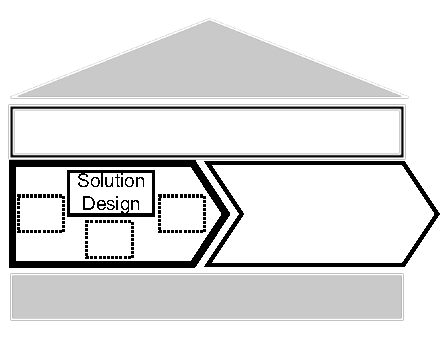
\includegraphics{figures/processes/solutiondesign.pdf}
			\end{center}
		\end{subfigure}
		\begin{subfigure}[c]{.45\textwidth}
			\begin{center}
				\begin{tikzpicture}
				[node distance=.4cm, start chain=going below,font=\sffamily]
				\node[punktchain, rounded corners=0pt, join=by {-}] (eins)      {process service definition};
				\node[punktchain, rounded corners=0pt, join=by {-}] (zwei)      {match product};
				\node[punktchain, rounded corners=0pt, join=by {-}] (drei)      {specify solution};
				\node[punktchain, rounded corners=0pt, join=by {-}] (vier)      {develop solution};
				\node[punktchain, rounded corners=0pt, join=by {-}] (fuenf)      {deliver solution};
				
				\end{tikzpicture}
			\end{center}
		\end{subfigure}
		
	\end{figure}
	
	\subsubsection{Process Service Definition}
	The first two detail processes represent the \textit{Discover} phase of the double diamond process. Its purpose is to identify the problem or needs to be addressed through design. In this case, the client's service definition object originates from the \textsc{Sales} process and holds requirements. However, these requirements will define the solution space, but not the concrete service (solution). The \acrshort{DDDP} proposes tools like customer journey maps to understand and discover the problem. This tool is seen as a very helpful means, as in context of omni-channel the customer experience can be mapped across different contact channels. Outcome of this detail process is a formalization of the client's problem that is used in the following detail process. 
	
	\subsubsection{Match Product}
	Products of the service provider are managed in the portfolio. In this detail process, the identified problem is used to match an existing product. Requirements regarding used systems in the provider's setting need to be included into this selection process. If no applicable product is found and the identified problem is deemed a reasonable addition to the portfolio (\ie it addresses a market demand), the \textsc{Product Development} process can be initiated. 
	
	\subsubsection{Specify Solution}
	This detail process relates to the \textit{Define} phase of the \acrshort{DDDP}. The matched product is now fitted to the problem, which results in a limited number of preliminary solutions. The idea is to get an estimate of the product's application in the client's context, so that an offer can be created in the \textsc{Sales} process. As the outsourcing deal is not closed at this point in time, the concrete implementation is not taking place in this detail process. 
	
	\subsubsection{Develop Solution}
	Development necessitates a commitment of the client, so that the efforts of implementing the solution are not in vain. Taking the process, people and technology perspective of \acrshort{CRM} or \acrshort{BPO}, these aspects do also apply on a solution. The importance of the different aspects may vary, as self-service solutions do require more focus on technology, while staffing is driving solutions with direct \acrshort{CSR} involvement. Outcome of this detail process is a detailed design of the solution's components. 
	
	\subsubsection{Deliver Solution}
	
	The last detail process finalizes the solution and eventually integrates it into \textsc{Transition}. A feedback mechanism to the portfolio shares insights of the product application to improve further use. Final testing, evaluation and approval are required before completing the \textsc{Solution Design} process. It relates to the fourth phase of the \acrshort{DDDP}.
	
	%%%%%%%%%%%%%%%%%%%%%%%%%%%%%%
	
	
	%	kurzer schwenk zu soziotechnischen systemen -> core IS einleitung?
	
	
	%	in outsourcing ist diese komponente variabel (kunden können system auch mitbringen)
	%die systemkomponente wird von den providern beigefügt, um die dienstleistung zu realisieren. system werden nicht %entwickelt. wohl aber services (und dementsprechend dann auch solutions)
	
	
	
	
	%	service design prozess: double diamond process. warum? gut für CJ (wichtig für omni-channel)
	%	Viewing the service design process from the service designer perspective
	
	%	requirements sind in der service definition zu finden, die im sales prozess übermittelt werden. 
	
	
	
	%	def solution, def product, def service architecture, service product, service konfiguration.  bottom up (sd, pd, pm)
	%	ref zu product development und so ... 
	
	
	\section{Management Processes}
	
	The third group of processes is located in the upper bar of the framework that represents their managerial aspect across the organization. The first two processes, \textsc{Product Development} and \textsc{Portfolio Management} work closely together with \textsc{Solution Design} and are hence oriented towards the client market. 
	
	\textsc{Quality Management} monitors operational service delivery for two purposes. On the one hand, it benchmarks processes across client businesses and ensures that the provider's operational capability is sustained. On the other hand, it represents reporting of service quality to existing client businesses.
	
	As \acrshort{BPO} is a labor intensive field, \textsc{People Lifecycle Management} fosters the provider's relationship to its customer service representatives. Their individual development is central part of the process and thereby contrasts the control-oriented view of work seen in \textsc{Operations Management}. The latter takes the business perspective that features planning and control of service delivery.
	
	Underlying process building blocks of management processes are not explicitly specified in this work, but suggestions for components are given in the textually. 
	
	\subsection{Product Development}
	\label{sec:proddev}
	
	As discussed in \ref{sec:soldef}, \acrshort{BPO} providers offer an integration of products and services for their clients, which are called solutions. In order to industrialize these customized solutions, the concept of modular service architectures from Service Engineering \citep{Bohmann2006} can be applied to structure into three levels: service architecture, service product and service configuration. These are represented in the framework through the portfolio (management process), product (development process) and solution (design process), respectively. \Fig \ref{fig:prodstructure} represents their interplay as an \acrshort{ERM}. 
	
	\begin{figure}[caption={Solution-Product-Portfolio Structure }, label={fig:prodstructure}]
		{	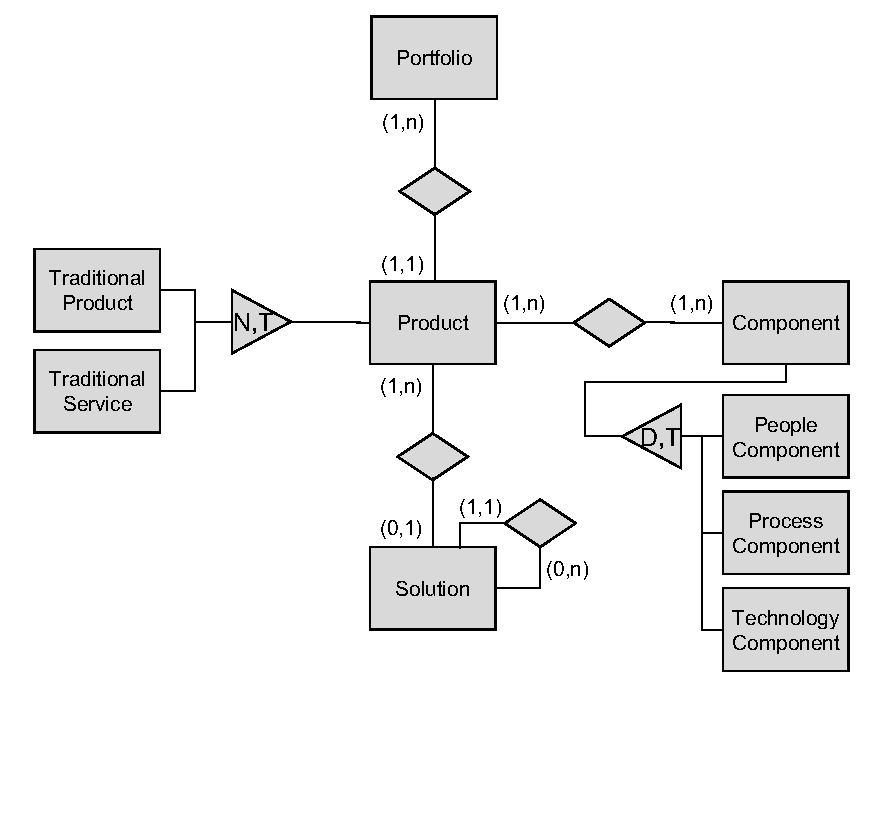
\includegraphics[width=.8\textwidth]{figures/producterm.pdf}}
		
	\end{figure} 
	
	The service architecture assures that service products or configurations are performing efficiently by maintaining their modular constituents, which are products and components. The service product puts together modules of the service architecture and targets specific markets. These are then configured towards a client, which is called a solution in this thesis. 
	
	Core of this process is to create new products that address a market need \wrt an existing portfolio. The defining object of this process is a product. In contrast to \textsc{Solution Design}, this process starts with a market perspective and therefore justifies the selection of a New Product/Service Development perspective.  
	
	Servitization makes clear boundaries between the traditional interpretations of services and products blurry. Like a solution, a product is always composed of both parts. The term product is used here to emphasize the orientation towards markets and therefore a \textit{standardization}, which is not given for client-specific solutions. \acrshort{BPO} providers do not manufacture a good, which is why a service-dominant perspective must be taken.  
	
	A plethora of product development processes, activities and frameworks exist in literature. The work of  \cite{cooper1988new} is seen as very influential in New Product Development. Adaptions for development of services are existing \citep{Edgett_1996}. Moreover, a dedicated framework for New Service Development is presented in \citep{cowell1988new}. A tabular comparison of their constituents is located in Appendix \ref{app:pdframeworks} and serves as basis for the process structure. 
	
	 \textsc{Product Development} starts with an idea. As idea generation can take place in various ways and is creative in its nature, the benefits of including it in a process model can be questioned. However, the screening of ideas can be structured more clearly, because a process that enables a standardized way of \textit{evaluating ideas} is meaningful. The complete process is shown in \Fig \ref{fig:pd} and continues with a market and technical assessment as proposed by \citep{Edgett_1996}, which subsumes the third section in \ref{app:pdframeworks}. The following detail processes are based on \citep{cowell1988new}. 
	
	
	\begin{figure}[caption={\textsc{Product Development }Process}, label={fig:pd}]
		\begin{subfigure}[c]{.45\textwidth}
			\begin{center}
				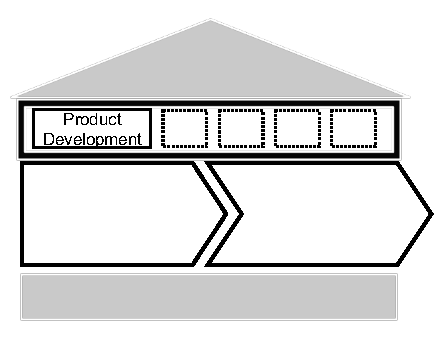
\includegraphics{figures/processes/productdevelopment.pdf}
			\end{center}
		\end{subfigure}
		\begin{subfigure}[c]{.45\textwidth}
			\begin{center}
				\begin{tikzpicture}
				[node distance=.4cm, start chain=going below,font=\sffamily]
				\node[punktchain, rounded corners=0pt, join=by {-}] (eins)      {evaluate idea};
				\node[punktchain, rounded corners=0pt, join=by {-}] (zwei)      {assess market requirements};
				\node[punktchain, rounded corners=0pt, join=by {-}] (drei)      {assess technical requirements};
				\node[punktchain, rounded corners=0pt, join=by {-}] (vier)      {conceptualize product};
				\node[punktchain, rounded corners=0pt, join=by {-}] (fuenf)      {perform business analysis};
				\node[punktchain, rounded corners=0pt, join=by {-}] (fuenf)      {develop product};
				\node[punktchain, rounded corners=0pt, join=by {-}] (fuenf)      {test product};
				\node[punktchain, rounded corners=0pt, join=by {-}] (fuenf)      {deliver product};
				\end{tikzpicture}
			\end{center}
		\end{subfigure}
		
	\end{figure}
	
	\subsubsection{Evaluate Idea}
	This first detail process has the aim to give decision support for an initial go/no go decision \wrt an idea for a new product, \ie whether to allocate resources for a deeper analysis. The formulation of evaluation criteria is an important step, with need to be aligned with business objectives and with respect to the portfolio. A product idea that solves a problem that is already addressed by another product in the portfolio might not be continued. An approval enables proceeding to the next detail process. 
	\subsubsection{Assess  Market Requirements}
	With an initial go decision being made, an investigation into market requirements is performed to evaluate whether a demand exists. \cite{Edgett_1996} splits this step further into a preliminary, nonscientific assessment and market research, which are both seen as part of this detail process. With respect to the domain, market requirements can originate from a client or customer perspective. 
	\subsubsection{Assess Technical Requirements}
	This detail process investigates into the question \textit{how} a product must be constituted to perform its task. The aspects people, process and technology can instance this from a \acrshort{CRM} point of view. In terms of technology, a product may be more or less limited to certain systems that provide required functionality. People, \ie, \acrshort{CSR}s, may need a certain skill set. Lastly, requirements regarding processes can play a role for quality standards, regarding legal issues or for realization of efficiency gains.
	
	\subsubsection{Conceptualize Product}
	The translation of requirements into a product concept is captured in this detail process. It brings together market  and technical requirements in order to create a preliminary design, which is more detailed than the idea in the beginning. It enables a more thorough reflection on the portfolio in two ways. On the one hand, its fit can be compared to existing products, \ie, towards the provider's offerings for clients. On the other hand, the concept can be assessed regarding its components and therefore its fit in the service architecture.
	
	\subsubsection{Perform Business Analysis}
	After a concept is existing, a detailed analysis leads to a final go/no go decision ahead of the actual product development. Aspects can include the attractiveness of the product concept, its chances of failure, required resources, costing or the response of competitors \citep[\p{302}]{cowell1988new}. Insights of the concept's fit regarding the service architecture, (\ie, portfolio) provide data for cost estimation and its practicability. 
	
	\subsubsection{Develop Product}
	Analogous to the \textit{develop solution} detail process in \textsc{Solution Design}, the transformation of the concept into a marketable product is constituting this step. As a product is developed without aiming at a specific client business, it needs to utilize abstraction as a means for enabling an application in different scenarios. However, the degree of abstraction depends on the product's integration into other \acrshort{CRM} systems, \ie, its ability to work stand-alone. The trade-off between implementation effort in a solution and abstraction needs to be considered: the more abstract a product, the less simple is its application in a solution. 
	
	\subsubsection{Test Product}
	The reason for modeling an explicit testing detail process in \textsc{Product Development} in contrast to \textsc{Solution Design} is seen in the fact that a product is always the basis of a solution. Consequently, a product needs to be assessed for its quality, reliability and performance in a rigorous manner as there is no related data existing. Solution testing can build on product testing. 
	
	\subsubsection{Deliver Product}
	Reusing the terminology of \textsc{Solution Design}, the final detail process passes the final product into the portfolio. In addition to the actual product, marketing material and documentation needs to be created that enables use in the \textsc{Sales} and \textsc{Solution Design} process, respectively. 
	
	%SD: viewing it from the designer perspective
	
	%	NSD: marketing- getrieben. passt hier besser. deshalb auch product development. produkte im sinne eines bpo providers verstehen. 
	
	%	new product development 
	
	\subsection{Portfolio Management}
	\label{sec:portmang}
	
	Drawing on the structure of solutions, products and components presented in the \acrshort{ERM} in \Fig \ref{fig:prodstructure}, the portfolio joins together products and components. It is the defining objective of the process and manages resource allocation so that existing products are aligned to the provider's business and technological objectives. In order to raise synergies across client businesses, the reuse of components becomes important. 
	
	\cite{cooper1999new} name four reasons why portfolio management is vital to business performance. First, portfolio management has a strategic component, as it operationalizes business strategy through the products and technologies that are chosen to be in focus. Second, these choices affect the future development and positioning of the company,\eg, enabling the addressing of omni-channel developments as a trend in \acrshort{CRM}. Third, Portfolio Management helps to allocate scarce resources like R\&D. Finally, a balancing of resources between products and components assures the right size and focus of the portfolio.     
	
	With respect to Service Engineering, the portfolio realizes a service architecture  \citep{Bohmann2006} by holding components that form products. The management of components serves internal purposes, so that reuse and combination increases efficiency. The management of products serves external purposes towards the client market. 
	
	The extensive definition of portfolio management \citep[\p{335}]{cooper1999new} located in Appendix \ref{app:pmdef} serves as a foundation for the process model in \Fig \ref{fig:portmang}. 
	
	
	\begin{figure}[caption={\textsc{Portfolio Management} Process}, label={fig:portmang}]
		\begin{subfigure}[c]{.36\textwidth}
			\begin{center}
				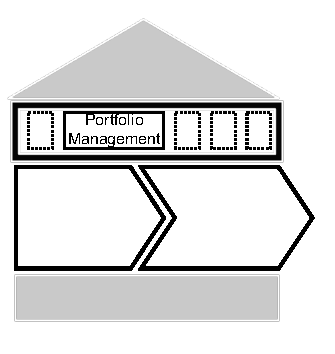
\includegraphics{figures/processes/portfoliomanagement.pdf}
			\end{center}
		\end{subfigure}
		\begin{subfigure}[c]{.6\textwidth}
			\begin{center}
				\begin{tikzpicture}
				[node distance=.4cm, start chain=going below,font=\sffamily]
				\node[punktchain, rounded corners=0pt, join=by {-}] (eins)      {maintain product};
				\node[punktchain, rounded corners=0pt, join=by {-}] (zwei)      {maintain component};
				\node[punktchain, rounded corners=0pt, join=by {-}] (drei)      {evaluate portfolio};
				\node[punktchain, rounded corners=0pt, join=by {-}] (vier)      {prioritize portfolio};
				\node[punktchain, rounded corners=0pt, join=by {-}] (fuenf)      {balance resources};
				\node[punktchain,rounded corners=0pt,  draw=white] (aux1) { };
				\node[punktchain,rounded corners=0pt,  below right=0.4cm and -2cm of fuenf] (konk) {terminate component};
				\node[punktchain, rounded corners=0pt,  left = of konk,] (konk2) {terminate product};
				\node[punktchain, rounded corners=0pt, below= of aux1, ] (sieben)      {update portfolio};
				\draw[|-,-|,-, thick,] (fuenf.south) |-+(0,-0.2cm)-| (konk.north);
				\draw[|-,-|,-, thick,] (fuenf.south) |-+(0,-0.2cm)-| (konk2.north);
				\draw[|-,-|,-, thick,] (konk.south) |-+(0,-0.2cm)-| (sieben.north);
				\draw[|-,-|,-, thick,] (konk2.south) |-+(0,-0.2cm)-| (sieben.north);
				\end{tikzpicture}
			\end{center}
		\end{subfigure}
		
	\end{figure}
	
	
	\subsubsection{Maintain Product}
	Products are one of two entities that compose the portfolio. While the \textsc{Product Development} process describes the creation of new products and its components with respect to the portfolio, updates of existing products are captured in this detail process. Feedback from solutions can be one trigger to update a product, as well as changes in its assignment of components. 
	
	The reason for locating the maintenance of product and components in a sequence lies in their relationship to each other. Correspondent to manufacturing, the product can be seen as the final item, while it is made out of parts and assemblies (components). The planning\footnote{It is noted that planning and maintaining are different activities. However, both activities have implications on products.} of sold items is made first and then the requirements of assemblies and parts is derived, because the former is market-oriented unlike the latter. 
	
	\subsubsection{Maintain Component}
	Three distinct types of components are defined (people, process, technology). Updates of existing technological components may be invoked by new versions of \acrshort{CRM} systems. Also the creation of new components is possible apart from \textsc{Product Development}, for instance when a new process component is created to perform additional data validity checking. The components regarding people represent the requirements \wrt service employees like their skill set. Lastly, the maintenance of component usage in products is another aspect of this detail process. 
	
	Objective of these first two detail processes is the guarantee of correct and complete information in the portfolio.
	
	\subsubsection{Evaluate Portfolio}
	There are different methods available to assess the quality of a portfolio and especially its constituents through numeric values. It is desisted from explicitly splitting the evaluation for products and components, as the portfolio as a whole needs to be examined. In the study of \cite{cooper1999new} the adoption of different methodologies is assessed. Dominating are financial methods, utilizing business strategy, scoring models, bubble diagrams and checklists. A typical business relies on 2.4 methods for managing their portfolio. The financial methods use profitability, return or net present value for scoring entities and is used in 77.3\% of cases. The alignment with business strategy determines the score in the second case and is used in 64.8\% of cases. Bubble diagrams utilize a plot with different measures of interest to structure their ratings in 40.6\%. Scoring models create various scales that form together one value for an entity and make up 37.9\%. Lastly, the checklist method accounts for 20.9\% and states a list of yes/no questions to be filled out for every entity.  
	
	Different employed methods imply different process details, but all methods have the goal to derive measures that can be used for prioritization. Outcome of this detail process are scores for the portfolio's constituents. 
	
	\subsubsection{Prioritize Portfolio}
	Building on the prior evaluation, this step \enquote{determines the order for dealing with a series of items according to their relative importance} \citep{oxfordprioritize}. With respect to the two entities, products and components need to be prioritized separately and the interchangeability of components has to be taken into account. Prioritizing is required for the following balancing detail process. 
	\subsubsection{Balance Resources}
	By definition, a business has to operate under scarce resources (\eg, time, capital, human resources). With respect to portfolio and prioritization of its constituents, these resources are allocated to products and components. This limits the number of products that can be part of the portfolio, as well as components that make up these products. When a component or product is not able to allocate the required resources, it cannot be sustained in the portfolio.
	This leads to the termination of the respective entity.
	
	\subsubsection{Terminate Product, Component}
	The exclusion of a product or component from the portfolio triggers its removal in operations. The termination is not  possible instantaneously \wrt components, as replacements need to be found and adapted. However, products do not have a superordinate element and can therefore be removed from the provider's offering with less interdependencies. As solutions do not necessarily depend on products (\cf \Fig \ref{fig:prodstructure}), they can persist even when their parent product is terminated. 
	
	
	\subsubsection{Update Portfolio}
	The termination of products and components is likely requiring updates in the portfolio, especially \wrt the assignments. As the process is completed with this step, it is necessary to communicate the updated portfolio to its stakeholders. 
	
	\subsection{Quality Management}
	\label{sec:qualmang}
	
	Quality management is an important issue in outsourcing. Poor service quality is the second highest ranked reason for clients having dispute with providers \citep{deloitte2014outsourcing}. Investments in quality monitoring are seen as most important in a recent study among contact centers \citep{ccnet2016}. Providers need to ensure their quality in service provision to stay competitive. From an internal perspective, a global quality management ensures comparability between and facilitates improvement across client businesses. Externally, the reporting of service quality in terms of \acrshort{SLA} is a focal requirement for providers. While this would also reason locating it in the client-oriented processes, internal quality management is seen as the paramount purpose of the process. 
	
	A broad definition of service quality shall be used in this context. Services are heterogeneous by definition \citep{cowell1988new}, so that an assessment cannot reference to a standard. In addition, the customer's opinion regarding quality is subjective and must be collected explicitly. To operationalize quality management, performance measures are used in addition in outsourcing, so that a quick response to a customer inquiry is assumed to relate to good quality.
	
	Considering quality management philosophies, one can name six sigma and \acrshort{TQM} and lean management \citep{Andersson_2006}. All are originating from manufacturing but have increasingly been adopted for service businesses \citep{Antony_2007}. It is not intention of the reference model to dictate the management approach, that goes hand in hand with selection of one of these concepts. Therefore, no recommendation to choose one philosophy over the other is made. However, the different methodologies in these are compared to derive a process structure applicable to the reference model. 
	
	\acrshort{TQM} proposes a split into four phases: plan (1), do (2), check (3), act(4). Six sigma lists define (1), measure (2), analyze (3), improve (4) and control (5). Shorthands are \acrshort{PDCA} and \acrshort{DMAIC}, respectively. Lean management does not provide such phases, which reasons its disqualification regarding process structuring. Both \acrshort{PDCA} and \acrshort{DMAIC} are designed as cycles. 
	
	In \acrshort{TQM} \textit{planning} of the initiative is important in order to identify objectives and potentials for improvement. \textit{Doing} represents a small scale testing of changes, which are \textit{checked} in the following phase. \textit{Act} describes the large-scale implementation of improvements that have previously been identified and starts the next cycle. 
	
	Six sigma contains a more granular view. First, the scope and objectives are \textit{defined}. Next, \textit{measuring} establishes the current baseline quality level by collecting service quality data, which is not explicitly part of the \acrshort{TQM} methodology. \textit{Analysis} identifies roots and causes of problems, which are then \textit{improved} in the fourth phase. As there is no equivalent to the small-scale doing and checking of \acrshort{TQM} in six sigma, an own \acrshort{PDCA} cycle can be a methodology for testing improvements in six sigma \citep{9780071840538}. The last phase, \textit{control}, sustains the quality gains and has a monitoring function.
	
	Icebricks process structure dictates that a main process (\textsc{Quality Management}) is made of detail processes, which consist of process building blocks. Consequently two layers of abstraction are left to be defined. A detail process structuring according to \acrshort{TQM} would result in rather abstract steps that then would have to be detailed completely on process building block level. However, using \acrshort{DMAIC} on detail process level conveys more details that can be specified on the lowest level. Therefore \textsc{Quality Management} is structured according to \acrshort{DMAIC}. 
	
	\begin{figure}[caption={\textsc{Quality Management} Process}, label={fig:qualmang}]
		\begin{subfigure}[c]{.36\textwidth}
			\begin{center}
				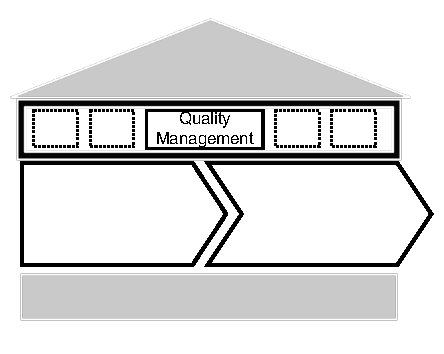
\includegraphics{figures/processes/qualitymanagement.pdf}
			\end{center}
		\end{subfigure}
		\begin{subfigure}[c]{.6\textwidth}
			\begin{center}
				\begin{tikzpicture}
				[node distance=.4cm, start chain=going below,font=\sffamily]
				\node[punktchain, rounded corners=0pt, join=by {-}] (eins)      {define service scope};
				\node[punktchain, rounded corners=0pt, join=by {-}] (zwei)      {measure service quality data};
				\node[punktchain, rounded corners=0pt, join=by {-}] (drei)      {analyze service quality data};
				\node[punktchain, rounded corners=0pt, join=by {-}] (fuenf)      {improve service quality};
				\node[punktchain,rounded corners=0pt,  draw=white] (aux1) { };
				\node[punktchain,rounded corners=0pt,  below right=0.5cm and -2cm of fuenf] (konk) {report service quality};
				\node[punktchain, rounded corners=0pt,  left = of konk,] (konk2) {control service quality};
				%	\node[punktchain, rounded corners=0pt, below= of aux1, ] (sieben)      {update portfolio};
				\draw[|-,-|,-, thick,] (fuenf.south) |-+(0,-0.5em)-| (konk.north);
				\draw[|-,-|,-, thick,] (fuenf.south) |-+(0,-0.5em)-| (konk2.north);
				%	\draw[|-,-|,-, thick,] (konk.south) |-+(0,-0.5em)-| (sieben.north);
				%	\draw[|-,-|,-, thick,] (konk2.south) |-+(0,-0.5em)-| (sieben.north);
				
				
				\end{tikzpicture}
			\end{center}
		\end{subfigure}
	\end{figure}
	
	\subsubsection{Define Service Scope}
	The first detail process has the purpose to frame carried out activities by selecting a service process (or part thereof), measures (\acrshort{KPI}s) that are used to assess quality and objectives to be achieved. These characteristics are seen as parts of the service scope, which justifies its selection as an umbrella term. For reporting of service quality an organizational dimension can be added (entire client business, a certain location, a certain channel). 
	\subsubsection{Measure Service Quality Data}
	After setting the scene, operative data needs to be captured in order to gain insights into the as-is performance. A common misconception in utilizing quality management approaches in services is that their origin in manufacturing limits their applicability in services due to \textit{noise} during service delivery \citep{Antony_2007}. While the statement that manufacturing services are more structured and less influenced by an uncontrollable factor is affirmed, especially outsourced services imply a degree of standardization that renders this fear misplaced. 
	
	Service quality data can be seen in explicit feedback by the customer or proxies in form of performance measures. Calculations of \acrshort{KPI}s like \acrfull{AHT} are a common aggregated measure to express the time required to solve a customer inquiry. In addition to these measures, information from systems and users (\acrshort{CSR}s) needs to be gathered for the upcoming analysis, because the identification of causes requires process details. It has to be noted that this performance measurement  also puts pressure on \acrshort{CSR}s and cause for dissatisfaction, stress and burnout \citep[\pf {678}]{Aksin_2009}, which reasons the necessity of \textsc{People Lifecycle Management}.
	
	\subsubsection{Analyze Service Quality Data}
	With the service quality data being available, its analysis can serve two purposes. First, it consolidates the information into a desirable format or structure (for example through aggregation to a contact center-level). Second, internal quality improvement requires an investigation in records or parts to identify problems, which does not necessarily have to be performed in service quality reporting. 
	
	\subsubsection{Improve Service Quality}
	Building on the analysis, this step can be seen as optional in case of service quality reporting to clients. Goal is to conduct a change so that the selected quality measure changes to the better. It might be necessary to discuss these changes with the client beforehand. The global perspective of \textsc{Quality Management} demands abstraction and sharing of gains with the organization, so that other client businesses can benefit. This requires a standardized service delivery process for which this reference model is a means. 
	
	As previously mentioned, the \acrshort{PDCA}-methodology can be used on process building block level to test and evaluate improvements. Outcome of this detail process is the changed process employing the \textit{optimal} configuration \wrt collected service quality data.  
	
	\subsubsection{Control \& Report Service Quality}
	These detail processes complete \textsc{Quality Management} with emphasis on the internal or external perspective. 
	Controlling keeps the internal perspective by managing consequences from service improvement (for example training of staff). Furthermore the monitoring of service quality is necessary to ensure the adoption of changes as new standards and their impact on overall performance.  
	The completion of the process in external use is seen in the reporting of service quality to the respective client. 
	
	\subsection{People Lifecycle Management}
	\label{sec:plmang}
	Research on dissatisfaction, stress and illness (especially burnout) among \acrshort{CSR}s is an established research field \citep[\pf{678}]{Aksin_2009}. Reasons for this can be seen in taking a Tayloristic control-oriented view of work. However, an organizational behavior perspective can be taken to center the employee in the process. This benefits not only human resources, but also contact center performance through ways that are not taken into account in operations management. Investments in HR development are seen as the second most important investment in contact centers \citep{ccnet2016}.
	
	\textsc{People Lifecycle Management} is seen as a management process, as the relationship towards service delivering employees across client business should be aligned to develop the operational capability of the provider. However, as they are working in context of a specific client business, special characteristics need to be considered (\eg, in job requirements and recruiting). 
	
	Contact centers facing burnout suffer from higher turnover, absenteeism and low performance \citep{Tuten_2004}. Economically speaking, turnover increases hiring costs and negatively impacts performance levels and new employees need to pass through a learning curve. Absenteeism causes under-staffing and therefore damages service quality through increased waiting times. Lastly, stressed employees inevitably show less performance over time, as the relationship between stress and performance may be visualized as an inverted-U \citep[\p{27}]{Tuten_2004}.
	
	Traditional, control-oriented, HR strategies do not adequately address this issues. Commitment strategies  \citep{Batt2002, Batt_2002}, featuring high-involvement practices towards employees, take a different perspective that is expressed in \textsc{People Lifecycle Management}. Selective hiring, extensive training, ongoing learning, incentives through training, job security and high pay levels as well as trust building measures are named as characteristics of a commitment strategy \citep{Batt2002}. The process is centered around the process object \textit{employee}, which is used instead of \acrshort{CSR} to emphasize its applicability beyond \acrshort{CRM} \acrshort{BPO}.
	
	Interpreting the belonging of an employee as a lifecycle process, one can identify a time-logical sequence. First, the company(\ie, provider) needs to \textit{attract employee talent}. This is followed by a \textit{recruiting} process that eventually finds and hires a new employee. In order to emphasize the social and technical aspect of starting a new job, \textit{training} and social \textit{integration} is modeled in two distinct and concurrent detail processes. Human resource \textit{development} accompanies the employee towards maturity in the lifecycle analogy. The company needs to give \textit{incentives} to continuously create firm-specific human capital and foster employee satisfaction, \eg, through job security, ongoing learning, compensations and trust-building performance management. As the relationship between employer and employee proceeds, \textit{employee retention} describes the trade-off between the senior employee's high performance and the firm's dependency on tacit knowledge. The lifecycle ends with the termination of the employment contract. 
	
	
	\begin{figure}[caption={\textsc{People Lifecycle Management} Process}, label={fig:plm}]
		\begin{subfigure}[c]{.36\textwidth}
			\begin{center}
				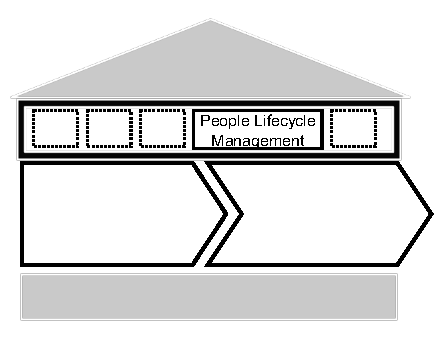
\includegraphics{figures/processes/plm.pdf}
			\end{center}
		\end{subfigure}
		\begin{subfigure}[c]{.60\textwidth}
			\begin{center}
				\begin{tikzpicture}
				[node distance=.4cm, start chain=going below,font=\sffamily]
				\node[punktchain, rounded corners=0pt, join=by {-}] (eins)      {attract employee talent};
				\node[punktchain, rounded corners=0pt, join=by {-}] (zwei)      {recruit employee};
				\node[punktchain,rounded corners=0pt,  draw=white] (aux1) { };
				\node[punktchain,rounded corners=0pt,  below right=0.4cm and -2cm of zwei] (t1) {integrate employee};
				\node[punktchain, rounded corners=0pt, left = of t1,] (t2) {train employee};
				\node[punktchain, rounded corners=0pt, below= of aux1, ] (sieben)      {develop employee};
				\node[punktchain, rounded corners=0pt, join=by {-} , ] (acht)      {incentivize employee};
				\node[punktchain, rounded corners=0pt, join=by {-} , ] (acht)      {retain employee};
				\node[punktchain, rounded corners=0pt, join=by {-} , ] (acht)      {let go employee};
				
				\draw[|-,-|,-, thick,] (zwei.south) |-+(0,-0.2cm)-| (t1.north);
				\draw[|-,-|,-, thick,] (zwei.south) |-+(0,-0.2cm)-| (t2.north);
				\draw[|-,-|,-, thick,] (t1.south) |-+(0,-0.2cm)-| (sieben.north);
				\draw[|-,-|,-, thick,] (t2.south) |-+(0,-0.2cm)-| (sieben.north);
				\end{tikzpicture}
			\end{center}
		\end{subfigure}
		
	\end{figure}
	
	\subsubsection{Attract Employee Talent}
		Selective hiring is named by \cite{Batt2002} in context of high-involvement HR practices and \cite{pfeffer1998seven} as one out of seven \textit{practices of successful} organizations. This approach has implications on the first two detail processes. Related to the detail process at hand, the applicant pool needs to be large enough, so that a thorough selection can take place in recruiting. The generation of this large application pool requires an attractive image towards potential employees to trigger generation of applications. \textit{Employee talent} as process object signifies that the company should state clearly what attributes and skills are required for the job. In \acrshort{BPO} these are specified by the targeted client business. The resulting volume in applications is input to the recruitment detail process. 
		
	\subsubsection{Recruit Employee}
		A rigorous recruitment process serves two purposes \citep[\p{101}]{pfeffer1998seven}. One the one hand, it ensures that the employee's fit towards the requirements is broadly assessed through tests and interviews. On the other hand, it proves the employee's commitment to the job offer. Cultural fit and attitude needs to be considered, as these factors can hardly be trained. It is also pointed out that hiring \enquote{the best and brightest} might not be the best choice for every job, as being overqualified has consequences in terms of retaining the employee the required time to reach break-even \wrt initial training and hiring costs. This detail process yields a new employee for the scoped client business.
	\subsubsection{Train Employee}
		An extensive training is necessary to ensure the required service quality expected from the employees as well as to lift the individual capacity to an average level. It can be seen as an upfront investment by the company. In customer service, proficiency in hard and soft skills is required to meet customer's expectations. 
	\subsubsection{Integrate Employee}
		Being seen as the second detail process of the \textit{onboarding} part of \textsc{People Lifecycle Management}, it represents the employee's social integration. Reason for this is to express the importance of the employee's relationship to peers, as well as the provider and client organization. Social integration addresses the employee's binding with the organization. Teams with a collaborative environment show better knowledge sharing capabilities that lead to better service \citep{Batt_2002}. Especially self-managed teams and decentralization are pointed out by \cite{pfeffer1998seven} as an effective principle. 
		
	\subsubsection{Develop Employee}
		After the employee reaches an operational performance level, a learning process starts. It is seen as a focal part of high-involvement HR to enable ongoing learning through collaboration with other employees \citep{Batt2002} (which necessitates integration beforehand). In contrast to initial training, the acquisition of new skills benefits  employee and provider through increased human capital. These can be formalized from individual skills into skill sets and be used to enable skill-based routing in service delivery. 
	\subsubsection{Incentivize Employee}
		Incentives act as a stimulus for employee motivation. Being one main aspect of high-involvement HR, job securities, promotions and fair payment are means provided by the company. Performance measurements can also be used to motivate the employee, while aiming for higher efficiency. 
	\subsubsection{Retain Employee}
	
	Turnover is an important issue in labor intensive services like \acrshort{CRM} \acrshort{BPO} \citep[\p{98}]{gross2006}. It is a management objective to find the right turnover rate, which depends on the knowledge of the workforce: When turnover rate is too low, knowledge can reside in employees which puts the company into dependency. An excessive turnover rate causes additional costs in recruiting and training, as the employee's individual return on investment decreases. \cite{Whitt2006} analyzes the relationship between employee retention on contact center performance. Higher satisfaction results to better retention, which leads to higher experience levels that positively impact performance. Knowing this trade-off  between performance and knowledge distribution is key in managing turnover rates.
	
	Consequently, this detail process typifies the company's strive for satisfied employees while limiting tacit knowledge. Exemplary activities are an evaluation of the employee's needs and knowledge. 
	
	\subsubsection{Let Go Employee}
	
	The final detail process describes separation of employee and company, which can be initiated by both sides. Knowledge transfer is important, because the provider must be able to adequately replace the position. Furthermore, feedback helps the organization to continuously improve its  \textsc{People Lifecycle Management}.
	
	
	
	\subsection{Operations Management}
	\label{sec:wofom}
	%Capacity Planning analogy als Einstieg.

		
	Operations management is the \enquote{activity of managing the resources which are devoted to the production and delivery of products and services} \citep[\p{4}]{0273708473}. Standardization of this fundamental and complex task in operations across client businesses bears great potential. Expert knowledge must be allocated at an overarching level in the provider organization. In this process, especially the activity planning and controlling the production is emphasized. A comparison of production planning\footnote{A plan refers to \enquote{a formalization of something that is intended to happen in future}\citep[\p{225}]{9780273756194}.} and control\footnote{Control is defined as \enquote{the adjustments which allow the operation to achieve the objectives that the plan has set, even when the assumptions on which the plan was based do not hold true.} \citep[\p{225}]{9780273756194}. } \citep{9780130176158} to its counterparts in \acrshort{CRM} service delivery signifies similarities between both fields. 
	The latter is in this case especially shaped by characteristics of contact centers. \cite{Aksin_2009} provides a  literature review from an operations management perspective. 

	In production planning, a master production schedule is created based on forecasts to outline the amount of end items required to meet market requirements. Transferring this to service provision requires forecasts of volume (demand) that needs to be addressed by service employees. In contrast to manufacturing, service capacity needs to be available concurrent to demand. 

	A master production schedule is broken down into a material requirements plan, which specifies parts that are needed to assembly an end item. Mirroring to services, service volume can be specified regarding channels, arrival distributions and service time distributions \citep{Aksin_2009}. It is noted that available literature focuses on classic call centers (\ie, voice channel only), which is abstracted from in this case. 
	
	As an additional layer of complexity, \acrshort{CSR}s must be seen as a different kind of operational resource in comparison to machinery in manufacturing. Individual skills, shift plans and employment law are only three factors that need to be considered in addition. \cite{Aksin_2009} lists staffing problems (1) and shift scheduling and rostering (2) in this regard. Ad (1), different queuing and simulation models are utilized to estimate targeted staffing levels \textit{for a period}, so that a cost minimal \acrshort{CSR} schedule that fulfills \acrshort{SLA}s can be derived. 
	(2) takes the results from staffing problems as inputs and seeks to create a detailed schedule on an interval basis. Rostering problems target combination of shifts into rosters to match them with \acrshort{CSR}s. Academic literature provides extensive research in this field \citep{Gans_2003, Ernst_2004}. 
	
	As forecasts are never correct and services are heterogeneous, a deviation between plan and reality will take place, which is taken care of on \textit{control} level. Here, sudden events must be managed and so that operational performance is sustained. 
	
	The structure of the \textsc{Operations Management} process is oriented towards production planning and control systems \citep{9780130176158} so that detail level increases and time horizon decreases over time, \viz as the process progresses. 
	%  Hence, it is started with a rough-cut planning to forecast a demand volume, because predictions are always more accurate when aggregated to a single number (\eg, overall volume instead of channel-specific volume). Based on this forecasts, the planning is continued and broken down so that a granular, daily schedule can be created that allocates \acrshort{CSR}s and to time slots, so that in sum the required capacity \wrt to the forecast is available.  
	
	\begin{figure}[caption={\textsc{Operations Management} Process}, label={fig:wfm}]
		\begin{subfigure}[c]{.45\textwidth}
			\begin{center}
				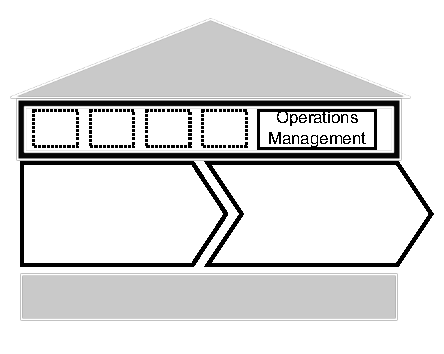
\includegraphics{figures/processes/operationsmanagement.pdf}
			\end{center}
		\end{subfigure}
		\begin{subfigure}[c]{.45\textwidth}
			\begin{center}
				\begin{tikzpicture}
				[node distance=.4cm, start chain=going below,font=\sffamily]
				\node[punktchain, rounded corners=0pt, join=by {-}] (eins)      {forecast service volume};
				\node[punktchain, rounded corners=0pt, join=by {-}] (zwei)      {plan capacity requirements};
				\node[punktchain, rounded corners=0pt, join=by {-}] (vier)      {plan schedule};
				\node[punktchain, rounded corners=0pt, join=by {-}] (fuenf)      {control operations};
				\end{tikzpicture}
			\end{center}
		\end{subfigure}
		
	\end{figure}
	
	\subsubsection{Forecast Service Volume}
	Different methods can be employed for creating predictions \citep{9780470525906}. Time-series forecasts can be one tool for predicting an outcome (volume) from time as single dependent variable. Defining characteristic of this detail process is that the granularity of these forecasts is covering up to weekly forecasts. Increased granularity is subject to following detail processes, that build on the forecasts being the output of this step. In outsourcing, these forecasts might be supplied by the client. \textit{Forecasting} as an activity is used to emphasize that this detail processes captures external demand and shows less connection to the actual planning of the operational business.
	
	\subsubsection{Plan Capacity Requirements}
	The breakdown of service volume is basis for planning of capacity requirements. Capacity expresses the amount of services that can be produced in a period. Capacity requirements record how many \acrfullpl{FTE} are needed and refer to a more granular view of service volume that takes into account service time and arrival distributions. 
	
	This detail processes addresses the staffing problem. Its complexity can be increase by dropping assumptions such as homogeneous agents and only one type of service, which has been addressed recently in literature \citep[\pf{699}]{Aksin_2009}. The capacity requirements are necessary for scheduling.
	
	\subsubsection{Plan Schedule}
	This detail processes encompasses addressing the scheduling and rostering problem. As there are a plethora of different methods and their discussion is beyond scope of this thesis, the reader is referred to  \citep[\pf{670}]{Aksin_2009} for an literature overview. The traditional split between scheduling and rostering problem is rejected in some methods, so is no further separation within this process. Result of this step is a plan that brings together staffed \acrshort{CSR}s on an intra-day schedule.
	
	\subsubsection{Control Operations}
	The execution of plans results in deviations that \textsc{Operations Management} must cope with. Drawing on the preceding scheduling, their adjustments on a real-time basis are an issue that has been addressed in literature \citep{Hur_2009, Easton_2005, Mehrotra_2009}. Over- and under-staffing situations result in excessive operational costs or violations of \acrshort{SLA}s due to customers waiting times. 
	
	While planning activities offer a higher potential of standardization across the organization, the execution and control is likely to be dependent on the business and location at hand. 
	
	%%%%%%%%%%
	%%%%%%%%%%